\documentclass[]{book}
\usepackage{lmodern}
\usepackage{amssymb,amsmath}
\usepackage{ifxetex,ifluatex}
\usepackage{fixltx2e} % provides \textsubscript
\ifnum 0\ifxetex 1\fi\ifluatex 1\fi=0 % if pdftex
  \usepackage[T1]{fontenc}
  \usepackage[utf8]{inputenc}
\else % if luatex or xelatex
  \ifxetex
    \usepackage{mathspec}
  \else
    \usepackage{fontspec}
  \fi
  \defaultfontfeatures{Ligatures=TeX,Scale=MatchLowercase}
\fi
% use upquote if available, for straight quotes in verbatim environments
\IfFileExists{upquote.sty}{\usepackage{upquote}}{}
% use microtype if available
\IfFileExists{microtype.sty}{%
\usepackage{microtype}
\UseMicrotypeSet[protrusion]{basicmath} % disable protrusion for tt fonts
}{}
\usepackage[margin=1in]{geometry}
\usepackage{hyperref}
\hypersetup{unicode=true,
            pdftitle={Introducción al software estadístico R},
            pdfauthor={Dae-Jin Lee \textless{} dlee@bcamath.org \textgreater{}},
            pdfborder={0 0 0},
            breaklinks=true}
\urlstyle{same}  % don't use monospace font for urls
\usepackage{natbib}
\bibliographystyle{apalike}
\usepackage{color}
\usepackage{fancyvrb}
\newcommand{\VerbBar}{|}
\newcommand{\VERB}{\Verb[commandchars=\\\{\}]}
\DefineVerbatimEnvironment{Highlighting}{Verbatim}{commandchars=\\\{\}}
% Add ',fontsize=\small' for more characters per line
\usepackage{framed}
\definecolor{shadecolor}{RGB}{248,248,248}
\newenvironment{Shaded}{\begin{snugshade}}{\end{snugshade}}
\newcommand{\KeywordTok}[1]{\textcolor[rgb]{0.13,0.29,0.53}{\textbf{#1}}}
\newcommand{\DataTypeTok}[1]{\textcolor[rgb]{0.13,0.29,0.53}{#1}}
\newcommand{\DecValTok}[1]{\textcolor[rgb]{0.00,0.00,0.81}{#1}}
\newcommand{\BaseNTok}[1]{\textcolor[rgb]{0.00,0.00,0.81}{#1}}
\newcommand{\FloatTok}[1]{\textcolor[rgb]{0.00,0.00,0.81}{#1}}
\newcommand{\ConstantTok}[1]{\textcolor[rgb]{0.00,0.00,0.00}{#1}}
\newcommand{\CharTok}[1]{\textcolor[rgb]{0.31,0.60,0.02}{#1}}
\newcommand{\SpecialCharTok}[1]{\textcolor[rgb]{0.00,0.00,0.00}{#1}}
\newcommand{\StringTok}[1]{\textcolor[rgb]{0.31,0.60,0.02}{#1}}
\newcommand{\VerbatimStringTok}[1]{\textcolor[rgb]{0.31,0.60,0.02}{#1}}
\newcommand{\SpecialStringTok}[1]{\textcolor[rgb]{0.31,0.60,0.02}{#1}}
\newcommand{\ImportTok}[1]{#1}
\newcommand{\CommentTok}[1]{\textcolor[rgb]{0.56,0.35,0.01}{\textit{#1}}}
\newcommand{\DocumentationTok}[1]{\textcolor[rgb]{0.56,0.35,0.01}{\textbf{\textit{#1}}}}
\newcommand{\AnnotationTok}[1]{\textcolor[rgb]{0.56,0.35,0.01}{\textbf{\textit{#1}}}}
\newcommand{\CommentVarTok}[1]{\textcolor[rgb]{0.56,0.35,0.01}{\textbf{\textit{#1}}}}
\newcommand{\OtherTok}[1]{\textcolor[rgb]{0.56,0.35,0.01}{#1}}
\newcommand{\FunctionTok}[1]{\textcolor[rgb]{0.00,0.00,0.00}{#1}}
\newcommand{\VariableTok}[1]{\textcolor[rgb]{0.00,0.00,0.00}{#1}}
\newcommand{\ControlFlowTok}[1]{\textcolor[rgb]{0.13,0.29,0.53}{\textbf{#1}}}
\newcommand{\OperatorTok}[1]{\textcolor[rgb]{0.81,0.36,0.00}{\textbf{#1}}}
\newcommand{\BuiltInTok}[1]{#1}
\newcommand{\ExtensionTok}[1]{#1}
\newcommand{\PreprocessorTok}[1]{\textcolor[rgb]{0.56,0.35,0.01}{\textit{#1}}}
\newcommand{\AttributeTok}[1]{\textcolor[rgb]{0.77,0.63,0.00}{#1}}
\newcommand{\RegionMarkerTok}[1]{#1}
\newcommand{\InformationTok}[1]{\textcolor[rgb]{0.56,0.35,0.01}{\textbf{\textit{#1}}}}
\newcommand{\WarningTok}[1]{\textcolor[rgb]{0.56,0.35,0.01}{\textbf{\textit{#1}}}}
\newcommand{\AlertTok}[1]{\textcolor[rgb]{0.94,0.16,0.16}{#1}}
\newcommand{\ErrorTok}[1]{\textcolor[rgb]{0.64,0.00,0.00}{\textbf{#1}}}
\newcommand{\NormalTok}[1]{#1}
\usepackage{longtable,booktabs}
\usepackage{graphicx,grffile}
\makeatletter
\def\maxwidth{\ifdim\Gin@nat@width>\linewidth\linewidth\else\Gin@nat@width\fi}
\def\maxheight{\ifdim\Gin@nat@height>\textheight\textheight\else\Gin@nat@height\fi}
\makeatother
% Scale images if necessary, so that they will not overflow the page
% margins by default, and it is still possible to overwrite the defaults
% using explicit options in \includegraphics[width, height, ...]{}
\setkeys{Gin}{width=\maxwidth,height=\maxheight,keepaspectratio}
\IfFileExists{parskip.sty}{%
\usepackage{parskip}
}{% else
\setlength{\parindent}{0pt}
\setlength{\parskip}{6pt plus 2pt minus 1pt}
}
\setlength{\emergencystretch}{3em}  % prevent overfull lines
\providecommand{\tightlist}{%
  \setlength{\itemsep}{0pt}\setlength{\parskip}{0pt}}
\setcounter{secnumdepth}{5}
% Redefines (sub)paragraphs to behave more like sections
\ifx\paragraph\undefined\else
\let\oldparagraph\paragraph
\renewcommand{\paragraph}[1]{\oldparagraph{#1}\mbox{}}
\fi
\ifx\subparagraph\undefined\else
\let\oldsubparagraph\subparagraph
\renewcommand{\subparagraph}[1]{\oldsubparagraph{#1}\mbox{}}
\fi

%%% Use protect on footnotes to avoid problems with footnotes in titles
\let\rmarkdownfootnote\footnote%
\def\footnote{\protect\rmarkdownfootnote}

%%% Change title format to be more compact
\usepackage{titling}

% Create subtitle command for use in maketitle
\newcommand{\subtitle}[1]{
  \posttitle{
    \begin{center}\large#1\end{center}
    }
}

\setlength{\droptitle}{-2em}

  \title{Introducción al software estadístico \texttt{R}}
    \pretitle{\vspace{\droptitle}\centering\huge}
  \posttitle{\par}
  \subtitle{\begin{quote}
Curso de formación Euskaltel
\end{quote}}
  \author{Dae-Jin Lee \textless{}
\href{mailto:dlee@bcamath.org}{\nolinkurl{dlee@bcamath.org}}
\textgreater{}}
    \preauthor{\centering\large\emph}
  \postauthor{\par}
      \predate{\centering\large\emph}
  \postdate{\par}
    \date{Marzo 2019}

\usepackage{booktabs}
\usepackage[spanish]{babel}
\usepackage{amsthm}
\makeatletter
\def\thm@space@setup{%
  \thm@preskip=8pt plus 2pt minus 4pt
  \thm@postskip=\thm@preskip
}
\makeatother

\begin{document}
\maketitle

{
\setcounter{tocdepth}{1}
\tableofcontents
}
\chapter{Información y
pre-requisitos}\label{informacion-y-pre-requisitos}

\begin{itemize}
\item
  \textbf{Requisitos:}

  \begin{itemize}
  \tightlist
  \item
    Última versión del software \texttt{R} (Download R)
  \item
    \texttt{Rstudio} (Download Rstudio).
  \end{itemize}
\end{itemize}

~

\begin{itemize}
\item
  \textbf{Horario:}

  \begin{itemize}
  \item
    Día 11 de marzo 10:30 a 14:30 horas
  \item
    Días 12 y 13 de marzo de 09.00 a 13.00 horas
  \item
    Día 14 de marzo 09.00 a 12.00 horas
  \end{itemize}
\end{itemize}

~

\begin{itemize}
\tightlist
\item
  \textbf{Objetivos del curso}
\end{itemize}

El curso proporcionará conocimientos básicos y habilidades para utilizar
\texttt{R} como entorno de trabajo. Para ello, el curso ofrecerá una
visión general de las herramientas ofrecidas por \texttt{R}, por
ejemplo, manejo de matrices y conjuntos de datos, ilustraciones
gráficas, pruebas y análisis estadísticos, programación en \texttt{R} y
técnicas de modelización estadística y aprendizaje automático.

El objetivo es que al final del curso todos se hayan familiarizado con
el software estadístico \texttt{R}.

\chapter{\texorpdfstring{Introducción al software estadístico
\texttt{R}}{Introducción al software estadístico R}}\label{intro}

\texttt{R} es un entorno de programación orientado al cálculo,
manipulación de datos, y representación gráfica, publicado como software
libre con licencia GNU-GPL.

~

\section{\texorpdfstring{Instalar un paquete de
\texttt{R}}{Instalar un paquete de R}}\label{instalar-un-paquete-de-r}

\begin{itemize}
\tightlist
\item
  Desde la consola
\end{itemize}

\begin{Shaded}
\begin{Highlighting}[]
\KeywordTok{install.packages}\NormalTok{(}\StringTok{"< Nombre del paquete >"}\NormalTok{)}
\end{Highlighting}
\end{Shaded}

\begin{itemize}
\tightlist
\item
  Ejemplo:
\end{itemize}

\begin{Shaded}
\begin{Highlighting}[]
\KeywordTok{install.packages}\NormalTok{(}\StringTok{"DAAG"}\NormalTok{)}
\KeywordTok{install.packages}\NormalTok{(}\KeywordTok{c}\NormalTok{(}\StringTok{"DAAG"}\NormalTok{,}\StringTok{"psych"}\NormalTok{)) }\CommentTok{# Varios paquetes con el comando c("< Paquete 1 >","< Paquete 2 >")}
\end{Highlighting}
\end{Shaded}

\begin{itemize}
\tightlist
\item
  Desde Rstudio: \texttt{Packages\ \textgreater{}\ Install}
\end{itemize}

\section{\texorpdfstring{Empezando con
\texttt{R}}{Empezando con R}}\label{empezando-con-r}

\begin{itemize}
\tightlist
\item
  Obtener el directorio de trabajo o \emph{working directory}
\end{itemize}

\begin{Shaded}
\begin{Highlighting}[]
\KeywordTok{getwd}\NormalTok{() }
\end{Highlighting}
\end{Shaded}

\begin{itemize}
\tightlist
\item
  listar los objetos en el espacio de trabajo o \emph{workspace}
\end{itemize}

\begin{Shaded}
\begin{Highlighting}[]
\KeywordTok{ls}\NormalTok{()}
\end{Highlighting}
\end{Shaded}

\begin{itemize}
\tightlist
\item
  Definir el \emph{working directory}
\end{itemize}

\begin{Shaded}
\begin{Highlighting}[]
\KeywordTok{setwd}\NormalTok{(}\StringTok{"/Users/dlee"}\NormalTok{) }
\end{Highlighting}
\end{Shaded}

\begin{itemize}
\tightlist
\item
  Ver los últimos comandos utilizados en la consola
\end{itemize}

\begin{Shaded}
\begin{Highlighting}[]
\KeywordTok{history}\NormalTok{() }\CommentTok{# mostrar los últimos 25 comandos}
\KeywordTok{history}\NormalTok{(}\DataTypeTok{max.show=}\OtherTok{Inf}\NormalTok{) }\CommentTok{# mostrar todos los comandos anteriores}
\end{Highlighting}
\end{Shaded}

\begin{itemize}
\tightlist
\item
  Guardar el historial de comandos
\end{itemize}

\begin{Shaded}
\begin{Highlighting}[]
\KeywordTok{savehistory}\NormalTok{(}\DataTypeTok{file=}\StringTok{"myfile"}\NormalTok{) }\CommentTok{# el valor por defecto es ".Rhistory"}
\end{Highlighting}
\end{Shaded}

\begin{itemize}
\tightlist
\item
  Cargar los commandos guardados en una sesión anterior
\end{itemize}

\begin{Shaded}
\begin{Highlighting}[]
\KeywordTok{loadhistory}\NormalTok{(}\DataTypeTok{file=}\StringTok{"myfile"}\NormalTok{) }\CommentTok{# el valor por defecto es ".Rhistory"}
\end{Highlighting}
\end{Shaded}

\begin{itemize}
\tightlist
\item
  Salvar todo el \textbf{workspace} en un fichero \texttt{.RData}
\end{itemize}

\begin{Shaded}
\begin{Highlighting}[]
\KeywordTok{save.image}\NormalTok{()}
\end{Highlighting}
\end{Shaded}

\begin{itemize}
\tightlist
\item
  Guardar objectos especificos a un fichero (si no se especifica la ruta
  en el ordenador, se guardará en el directorio actual de trabajo).
\end{itemize}

\begin{Shaded}
\begin{Highlighting}[]
\KeywordTok{save}\NormalTok{(}\OperatorTok{<}\NormalTok{object list}\OperatorTok{>}\NormalTok{,}\DataTypeTok{file=}\StringTok{"myfile.RData"}\NormalTok{) }
\end{Highlighting}
\end{Shaded}

\begin{itemize}
\tightlist
\item
  Cargar un \emph{workspace} en la sesión
\end{itemize}

\begin{Shaded}
\begin{Highlighting}[]
\KeywordTok{load}\NormalTok{(}\StringTok{"myfile.RData"}\NormalTok{) }
\end{Highlighting}
\end{Shaded}

\begin{itemize}
\tightlist
\item
  Salir de \texttt{R}. Por defecto \texttt{R} pregunta si deseas guardar
  la sesión.
\end{itemize}

\begin{Shaded}
\begin{Highlighting}[]
\KeywordTok{q}\NormalTok{()}
\end{Highlighting}
\end{Shaded}

\section{\texorpdfstring{Instalar y cargar librerías en
\texttt{R}}{Instalar y cargar librerías en R}}\label{instalar-y-cargar-librerias-en-r}

\begin{Shaded}
\begin{Highlighting}[]
\KeywordTok{install.packages}\NormalTok{(}\StringTok{"DAAG"}\NormalTok{) }\CommentTok{# (Data Analysis And Graphics)}
\end{Highlighting}
\end{Shaded}

\begin{itemize}
\tightlist
\item
  Una vez instalada la librería, tenemos que cargarla con el comando
  \texttt{library} o \texttt{require}
\end{itemize}

\begin{Shaded}
\begin{Highlighting}[]
\KeywordTok{library}\NormalTok{(DAAG) }\CommentTok{# o require(DAAG)}
\end{Highlighting}
\end{Shaded}

\section{Lectura de datos}\label{lectura-de-datos}

Consola de \texttt{R}

\begin{Shaded}
\begin{Highlighting}[]
\NormalTok{x <-}\StringTok{ }\KeywordTok{c}\NormalTok{(}\FloatTok{7.82}\NormalTok{,}\FloatTok{8.00}\NormalTok{,}\FloatTok{7.95}\NormalTok{) }\CommentTok{# c de "combinar"}
\NormalTok{x}
\end{Highlighting}
\end{Shaded}

\begin{verbatim}
## [1] 7.82 8.00 7.95
\end{verbatim}

Otra forma es mediante la función \texttt{scan()}

\begin{Shaded}
\begin{Highlighting}[]
\NormalTok{x <-}\StringTok{ }\KeywordTok{scan}\NormalTok{()  }\CommentTok{# introducir números seguidos de ENTER y terminar con un ENTER}
\DecValTok{1}\OperatorTok{:}\StringTok{ }\FloatTok{7.82}
\DecValTok{2}\OperatorTok{:}\StringTok{ }\FloatTok{8.00}
\DecValTok{3}\OperatorTok{:}\StringTok{ }\FloatTok{7.95}
\DecValTok{4}\OperatorTok{:}\StringTok{ }
\NormalTok{Read }\DecValTok{3}\NormalTok{ items}
\end{Highlighting}
\end{Shaded}

Para crear un vector de caracteres \texttt{""}

\begin{Shaded}
\begin{Highlighting}[]
\NormalTok{id <-}\StringTok{ }\KeywordTok{c}\NormalTok{(}\StringTok{"John"}\NormalTok{,}\StringTok{"Paul"}\NormalTok{,}\StringTok{"George"}\NormalTok{,}\StringTok{"Ringo"}\NormalTok{)}
\end{Highlighting}
\end{Shaded}

To read a character vector

\begin{Shaded}
\begin{Highlighting}[]
\NormalTok{id <-}\StringTok{ }\KeywordTok{scan}\NormalTok{(,}\StringTok{""}\NormalTok{)}
\DecValTok{1}\OperatorTok{:}\StringTok{ }\NormalTok{John}
\DecValTok{2}\OperatorTok{:}\StringTok{ }\NormalTok{Paul}
\DecValTok{3}\OperatorTok{:}\StringTok{ }\NormalTok{George}
\DecValTok{4}\OperatorTok{:}\StringTok{ }\NormalTok{Ringo}
\DecValTok{5}\OperatorTok{:}\StringTok{ }
\NormalTok{Read }\DecValTok{4}\NormalTok{ items  }
\end{Highlighting}
\end{Shaded}

\begin{Shaded}
\begin{Highlighting}[]
\NormalTok{id}
\end{Highlighting}
\end{Shaded}

\begin{verbatim}
## [1] "John"   "Paul"   "George" "Ringo"
\end{verbatim}

\section{Importar datos}\label{importar-datos}

En ocasiones, necesitaremos leer datos de un fichero independiente.
Existen varias formas de hacerlo:

\begin{itemize}
\tightlist
\item
  \texttt{scan()} (\texttt{?scan} ver la ayuda)
\end{itemize}

\begin{Shaded}
\begin{Highlighting}[]
\CommentTok{# creamos el fichero ex.txt}
\KeywordTok{cat}\NormalTok{(}\StringTok{"Example:"}\NormalTok{, }\StringTok{"2 3 5 7"}\NormalTok{, }\StringTok{"11 13 17"}\NormalTok{, }\DataTypeTok{file =} \StringTok{"ex.txt"}\NormalTok{, }\DataTypeTok{sep =} \StringTok{"}\CharTok{\textbackslash{}n}\StringTok{"}\NormalTok{) }
\KeywordTok{scan}\NormalTok{(}\StringTok{"ex.txt"}\NormalTok{, }\DataTypeTok{skip =} \DecValTok{1}\NormalTok{)}
\end{Highlighting}
\end{Shaded}

\begin{verbatim}
## [1]  2  3  5  7 11 13 17
\end{verbatim}

\begin{Shaded}
\begin{Highlighting}[]
\KeywordTok{scan}\NormalTok{(}\StringTok{"ex.txt"}\NormalTok{, }\DataTypeTok{skip =} \DecValTok{1}\NormalTok{, }\DataTypeTok{nlines =} \DecValTok{1}\NormalTok{) }\CommentTok{# only 1 line after the skipped one}
\end{Highlighting}
\end{Shaded}

\begin{verbatim}
## [1] 2 3 5 7
\end{verbatim}

\begin{Shaded}
\begin{Highlighting}[]
\KeywordTok{unlink}\NormalTok{(}\StringTok{"ex.data"}\NormalTok{) }\CommentTok{# tidy up}
\end{Highlighting}
\end{Shaded}

\begin{itemize}
\item
  Existen diferentes formatos (\texttt{.txt}, \texttt{.csv},
  \texttt{.xls}, \texttt{.xlsx}, \texttt{SAS}, \texttt{Stata},
  etc\ldots{})
\item
  Alguna librer?as de \texttt{R} para importar datos:
\end{itemize}

\begin{Shaded}
\begin{Highlighting}[]
\KeywordTok{library}\NormalTok{(gdata)}
\KeywordTok{library}\NormalTok{(foreign)}
\end{Highlighting}
\end{Shaded}

\bigskip

\begin{itemize}
\tightlist
\item
  Generalmente leeros datos en formato \texttt{.txt} o \texttt{.csv}
\end{itemize}

Descara en el siguiente link los datos \texttt{cardata}
\href{data/cardata.zip}{aquí}

\begin{Shaded}
\begin{Highlighting}[]
\NormalTok{mydata1 =}\StringTok{ }\KeywordTok{read.table}\NormalTok{(}\StringTok{"data/cardata.txt"}\NormalTok{) }
\NormalTok{mydata2 =}\StringTok{ }\KeywordTok{read.csv}\NormalTok{(}\StringTok{"data/cardata.csv"}\NormalTok{)  }
\end{Highlighting}
\end{Shaded}

\begin{itemize}
\tightlist
\item
  Otros formatos \texttt{.xls} and \texttt{.xlsx}
\end{itemize}

\begin{Shaded}
\begin{Highlighting}[]
\KeywordTok{library}\NormalTok{(gdata)}
\NormalTok{mydata3 =}\StringTok{ }\KeywordTok{read.xls}\NormalTok{ (}\StringTok{"cardata/cardata.xls"}\NormalTok{, }\DataTypeTok{sheet =} \DecValTok{1}\NormalTok{, }\DataTypeTok{header =} \OtherTok{TRUE}\NormalTok{)}
\end{Highlighting}
\end{Shaded}

\begin{itemize}
\tightlist
\item
  Minitab, SPSS, SAS or Stata
\end{itemize}

\begin{Shaded}
\begin{Highlighting}[]
\KeywordTok{library}\NormalTok{(foreign)                   }
\NormalTok{mydata =}\StringTok{ }\KeywordTok{read.mtp}\NormalTok{(}\StringTok{"mydata.mtp"}\NormalTok{)  }\CommentTok{# Minitab}
\NormalTok{mydata =}\StringTok{ }\KeywordTok{read.spss}\NormalTok{(}\StringTok{"myfile"}\NormalTok{, }\DataTypeTok{to.data.frame=}\OtherTok{TRUE}\NormalTok{) }\CommentTok{# SPSS}
\NormalTok{mydata =}\StringTok{ }\KeywordTok{read.dta}\NormalTok{(}\StringTok{"mydata.dta"}\NormalTok{) }\CommentTok{# Stata}
\end{Highlighting}
\end{Shaded}

\begin{itemize}
\tightlist
\item
  O tambi?n
\end{itemize}

\begin{Shaded}
\begin{Highlighting}[]
\KeywordTok{library}\NormalTok{(Hmisc)}
\NormalTok{mydata =}\StringTok{ }\KeywordTok{spss.get}\NormalTok{(}\StringTok{"mydata.por"}\NormalTok{, }\DataTypeTok{use.value.labels=}\OtherTok{TRUE}\NormalTok{)  }\CommentTok{# SPSS}
\end{Highlighting}
\end{Shaded}

\section{Exportar datos}\label{exportar-datos}

\begin{itemize}
\item
  Existen diferentes maneras de exportar datos desde \texttt{R} en
  diferentes formatos. Para SPSS, SAS y Stata. Por ejemplo, mediante la
  librería \texttt{foreign}. En Excel, la librería \texttt{xlsx}.
\item
  Texto delimitado por tabulaciones:
\end{itemize}

\begin{Shaded}
\begin{Highlighting}[]
\NormalTok{mtcars}
\NormalTok{?mtcars    }
\KeywordTok{write.table}\NormalTok{(mtcars, }\StringTok{"cardata.txt"}\NormalTok{, }\DataTypeTok{sep=}\StringTok{"}\CharTok{\textbackslash{}t}\StringTok{"}\NormalTok{) }
\end{Highlighting}
\end{Shaded}

\begin{itemize}
\tightlist
\item
  Hoja de cálculo de Excel:
\end{itemize}

\begin{Shaded}
\begin{Highlighting}[]
\KeywordTok{library}\NormalTok{(xlsx)}
\KeywordTok{write.xlsx}\NormalTok{(mydata, }\StringTok{"mydata.xlsx"}\NormalTok{)}
\end{Highlighting}
\end{Shaded}

\section{Vectores}\label{vectores}

\begin{itemize}
\item
  Descargar el siguiente código de \texttt{R}
  \href{http://idaejin.github.io/bcam-courses/rbasics/rbasics.R}{aquí}
\item
  Crear dos vectores
\end{itemize}

\begin{Shaded}
\begin{Highlighting}[]
\NormalTok{weight<-}\KeywordTok{c}\NormalTok{(}\DecValTok{60}\NormalTok{,}\DecValTok{72}\NormalTok{,}\DecValTok{57}\NormalTok{,}\DecValTok{90}\NormalTok{,}\DecValTok{95}\NormalTok{,}\DecValTok{72}\NormalTok{)  }
\KeywordTok{class}\NormalTok{(weight)}
\end{Highlighting}
\end{Shaded}

\begin{verbatim}
## [1] "numeric"
\end{verbatim}

\begin{Shaded}
\begin{Highlighting}[]
\NormalTok{height<-}\KeywordTok{c}\NormalTok{(}\FloatTok{1.75}\NormalTok{,}\FloatTok{1.80}\NormalTok{,}\FloatTok{1.65}\NormalTok{,}\FloatTok{1.90}\NormalTok{,}\FloatTok{1.74}\NormalTok{,}\FloatTok{1.91}\NormalTok{)}
\end{Highlighting}
\end{Shaded}

\begin{itemize}
\tightlist
\item
  calcular el Body Mass Index (\emph{índice de masa corporal})
\end{itemize}

\begin{Shaded}
\begin{Highlighting}[]
\NormalTok{bmi<-}\StringTok{ }\NormalTok{weight}\OperatorTok{/}\NormalTok{height}\OperatorTok{^}\DecValTok{2}
\NormalTok{bmi}
\end{Highlighting}
\end{Shaded}

\begin{verbatim}
## [1] 19.59184 22.22222 20.93664 24.93075 31.37799 19.73630
\end{verbatim}

\section{Estadística básica}\label{estadistica-basica}

\begin{itemize}
\tightlist
\item
  mean, median, st dev, variance
\end{itemize}

\begin{Shaded}
\begin{Highlighting}[]
\KeywordTok{mean}\NormalTok{(weight) }
\KeywordTok{median}\NormalTok{(weight)}
\KeywordTok{sd}\NormalTok{(weight)}
\KeywordTok{var}\NormalTok{(weight)}
\end{Highlighting}
\end{Shaded}

\begin{itemize}
\tightlist
\item
  Resumen de un vector
\end{itemize}

\begin{Shaded}
\begin{Highlighting}[]
\KeywordTok{summary}\NormalTok{(weight)}
\end{Highlighting}
\end{Shaded}

\begin{verbatim}
##    Min. 1st Qu.  Median    Mean 3rd Qu.    Max. 
##   57.00   63.00   72.00   74.33   85.50   95.00
\end{verbatim}

\begin{itemize}
\tightlist
\item
  o también
\end{itemize}

\begin{Shaded}
\begin{Highlighting}[]
\KeywordTok{min}\NormalTok{(weight)}
\KeywordTok{max}\NormalTok{(weight)}
\KeywordTok{range}\NormalTok{(weight)}
\KeywordTok{sum}\NormalTok{(weight)}
\KeywordTok{length}\NormalTok{(weight)}
\end{Highlighting}
\end{Shaded}

\begin{itemize}
\tightlist
\item
  Cuantiles y percentiles
\end{itemize}

\begin{Shaded}
\begin{Highlighting}[]
\KeywordTok{quantile}\NormalTok{(weight) }\CommentTok{# por defecto cuantil 25%, 50% y 75%}
\end{Highlighting}
\end{Shaded}

\begin{verbatim}
##   0%  25%  50%  75% 100% 
## 57.0 63.0 72.0 85.5 95.0
\end{verbatim}

\begin{Shaded}
\begin{Highlighting}[]
\KeywordTok{quantile}\NormalTok{(weight,}\KeywordTok{c}\NormalTok{(}\FloatTok{0.32}\NormalTok{,}\FloatTok{0.57}\NormalTok{,}\FloatTok{0.98}\NormalTok{))}
\end{Highlighting}
\end{Shaded}

\begin{verbatim}
##  32%  57%  98% 
## 67.2 72.0 94.5
\end{verbatim}

\begin{itemize}
\tightlist
\item
  Covarianza y correlación
\end{itemize}

La covarianza (\(\sigma_{xy}\)) indica el grado de variacion conjunta de
dos variables aleatorias respecto a sus medias

\begin{itemize}
\tightlist
\item
  Si \(\sigma_{xy}> 0\), hay dependencia directa (positiva), es decir, a
  grandes valores de \(x\) corresponden grandes valores de \(y\).
\item
  Si \(\sigma_{xy}= 0\), hay una covarianza 0 se interpreta como la no
  existencia de una relación lineal entre las dos variables estudiadas.
\item
  Si \(\sigma_{xy}< 0\)m hay dependencia inversa o negativa, es decir, a
  grandes valores de \(x\) corresponden peque?os valores de \(y\).
\end{itemize}

\[
\rm{Cov}(x,y) = \frac{1}{n}\sum_{i=1}^{n}(x_i - \bar{x})(y_i - \bar{y})
\]

\begin{Shaded}
\begin{Highlighting}[]
\KeywordTok{cov}\NormalTok{(weight,height)}
\end{Highlighting}
\end{Shaded}

\begin{verbatim}
## [1] 0.6773333
\end{verbatim}

El \emph{coeficiente de correlación} mide la relacion lineal (positiva o
negativa) entre dos variables. Formalmente es el cociente entre la
covarianza y el producto de las desviaciones t?picas de ambas variables.
Siendo \(\sigma_x\) y \(\sigma_y\) las desviaciones estandar y
\(\sigma_xy\) la covarianza entre \(x\) e \(y\).

\[
      \rho_{xy}  = \frac{\sigma_{xy}}{\sigma_x~\sigma_y}
\]

\begin{Shaded}
\begin{Highlighting}[]
\KeywordTok{cor}\NormalTok{(weight,height)}
\end{Highlighting}
\end{Shaded}

\begin{verbatim}
## [1] 0.437934
\end{verbatim}

\section{Vectores caracteres y variables
factor}\label{vectores-caracteres-y-variables-factor}

\begin{Shaded}
\begin{Highlighting}[]
\NormalTok{subject <-}\StringTok{ }\KeywordTok{c}\NormalTok{(}\StringTok{"John"}\NormalTok{,}\StringTok{"Peter"}\NormalTok{,}\StringTok{"Chris"}\NormalTok{,}\StringTok{"Tony"}\NormalTok{,}\StringTok{"Mary"}\NormalTok{,}\StringTok{"Jane"}\NormalTok{)}
\NormalTok{sex <-}\StringTok{ }\KeywordTok{c}\NormalTok{(}\StringTok{"MALE"}\NormalTok{,}\StringTok{"MALE"}\NormalTok{,}\StringTok{"MALE"}\NormalTok{,}\StringTok{"MALE"}\NormalTok{,}\StringTok{"FEMALE"}\NormalTok{,}\StringTok{"FEMALE"}\NormalTok{)}
\KeywordTok{class}\NormalTok{(subject)}
\end{Highlighting}
\end{Shaded}

\begin{verbatim}
## [1] "character"
\end{verbatim}

\begin{Shaded}
\begin{Highlighting}[]
\KeywordTok{table}\NormalTok{(sex)}
\end{Highlighting}
\end{Shaded}

\begin{verbatim}
## sex
## FEMALE   MALE 
##      2      4
\end{verbatim}

\section{Data frames}\label{data-frames}

\begin{Shaded}
\begin{Highlighting}[]
\NormalTok{Dat <-}\StringTok{ }\KeywordTok{data.frame}\NormalTok{(subject,sex,weight,height)}
\CommentTok{# a?adir el bmi a Dat}
\NormalTok{Dat}\OperatorTok{$}\NormalTok{bmi <-}\StringTok{ }\NormalTok{bmi  }\CommentTok{# o Dat$bmi <- weight/height^2}
\KeywordTok{class}\NormalTok{(Dat)}
\end{Highlighting}
\end{Shaded}

\begin{verbatim}
## [1] "data.frame"
\end{verbatim}

\begin{Shaded}
\begin{Highlighting}[]
\KeywordTok{str}\NormalTok{(Dat) }\CommentTok{# Ver la estructura del data.frame}
\end{Highlighting}
\end{Shaded}

\begin{verbatim}
## 'data.frame':    6 obs. of  5 variables:
##  $ subject: Factor w/ 6 levels "Chris","Jane",..: 3 5 1 6 4 2
##  $ sex    : Factor w/ 2 levels "FEMALE","MALE": 2 2 2 2 1 1
##  $ weight : num  60 72 57 90 95 72
##  $ height : num  1.75 1.8 1.65 1.9 1.74 1.91
##  $ bmi    : num  19.6 22.2 20.9 24.9 31.4 ...
\end{verbatim}

\begin{Shaded}
\begin{Highlighting}[]
\CommentTok{# cambiar el nombre de las filas}
\KeywordTok{rownames}\NormalTok{(Dat)<-}\KeywordTok{c}\NormalTok{(}\StringTok{"A"}\NormalTok{,}\StringTok{"B"}\NormalTok{,}\StringTok{"C"}\NormalTok{,}\StringTok{"D"}\NormalTok{,}\StringTok{"E"}\NormalTok{,}\StringTok{"F"}\NormalTok{)}

\CommentTok{# Acceder a los elementos del data.frame}
\NormalTok{Dat[,}\DecValTok{1}\NormalTok{]     }\CommentTok{# columna 1}
\end{Highlighting}
\end{Shaded}

\begin{verbatim}
## [1] John  Peter Chris Tony  Mary  Jane 
## Levels: Chris Jane John Mary Peter Tony
\end{verbatim}

\begin{Shaded}
\begin{Highlighting}[]
\NormalTok{Dat[,}\DecValTok{1}\OperatorTok{:}\DecValTok{3}\NormalTok{]   }\CommentTok{# columnas 1 a 3}
\end{Highlighting}
\end{Shaded}

\begin{verbatim}
##   subject    sex weight
## A    John   MALE     60
## B   Peter   MALE     72
## C   Chris   MALE     57
## D    Tony   MALE     90
## E    Mary FEMALE     95
## F    Jane FEMALE     72
\end{verbatim}

\begin{Shaded}
\begin{Highlighting}[]
\NormalTok{Dat[}\DecValTok{1}\OperatorTok{:}\DecValTok{2}\NormalTok{,]   }\CommentTok{# filas 1 a 2}
\end{Highlighting}
\end{Shaded}

\begin{verbatim}
##   subject  sex weight height      bmi
## A    John MALE     60   1.75 19.59184
## B   Peter MALE     72   1.80 22.22222
\end{verbatim}

\section{Trabajando con data frames}\label{trabajando-con-data-frames}

\textbf{Ejemplo: analizar datos por grupos}

\begin{itemize}
\tightlist
\item
  Obtener el peso (\texttt{weight}), altura (\texttt{height}) y
  \texttt{bmi} por \texttt{FEMALES} y \texttt{MALES}:
\end{itemize}

\begin{enumerate}
\def\labelenumi{\arabic{enumi}.}
\tightlist
\item
  Seleccionado cada grupo y calculando la media por grupos
\end{enumerate}

\begin{Shaded}
\begin{Highlighting}[]
\NormalTok{Dat[sex}\OperatorTok{==}\StringTok{"MALE"}\NormalTok{,]}
\NormalTok{Dat[sex}\OperatorTok{==}\StringTok{"FEMALE"}\NormalTok{,]}

\KeywordTok{mean}\NormalTok{(Dat[sex}\OperatorTok{==}\StringTok{"MALE"}\NormalTok{,}\DecValTok{3}\NormalTok{])  }\CommentTok{# weight average of MALEs}
\KeywordTok{mean}\NormalTok{(Dat[sex}\OperatorTok{==}\StringTok{"MALE"}\NormalTok{,}\StringTok{"weight"}\NormalTok{])}
\end{Highlighting}
\end{Shaded}

\begin{enumerate}
\def\labelenumi{\arabic{enumi}.}
\setcounter{enumi}{1}
\tightlist
\item
  Mediante la función \texttt{apply} por columnas
\end{enumerate}

\begin{Shaded}
\begin{Highlighting}[]
\KeywordTok{apply}\NormalTok{(Dat[sex}\OperatorTok{==}\StringTok{"FEMALE"}\NormalTok{,}\DecValTok{3}\OperatorTok{:}\DecValTok{5}\NormalTok{],}\DecValTok{2}\NormalTok{,mean)}
\KeywordTok{apply}\NormalTok{(Dat[sex}\OperatorTok{==}\StringTok{"MALE"}\NormalTok{,}\DecValTok{3}\OperatorTok{:}\DecValTok{5}\NormalTok{],}\DecValTok{2}\NormalTok{,mean)}

\CommentTok{# podemos utilizar la función apply con cualquier función}
\KeywordTok{apply}\NormalTok{(Dat[sex}\OperatorTok{==}\StringTok{"FEMALE"}\NormalTok{,}\DecValTok{3}\OperatorTok{:}\DecValTok{5}\NormalTok{],}\DecValTok{2}\NormalTok{,}\ControlFlowTok{function}\NormalTok{(x)\{x}\OperatorTok{+}\DecValTok{2}\NormalTok{\})}
\end{Highlighting}
\end{Shaded}

\begin{enumerate}
\def\labelenumi{\arabic{enumi}.}
\setcounter{enumi}{2}
\tightlist
\item
  función \texttt{by} o \texttt{colMeans}
\end{enumerate}

\begin{Shaded}
\begin{Highlighting}[]
\CommentTok{# 'by' divide los datos en factores y realiza }
\CommentTok{#   los cálculos para cada grupo}
\KeywordTok{by}\NormalTok{(Dat[,}\DecValTok{3}\OperatorTok{:}\DecValTok{5}\NormalTok{],sex, colMeans) }
\end{Highlighting}
\end{Shaded}

\begin{enumerate}
\def\labelenumi{\arabic{enumi}.}
\setcounter{enumi}{3}
\tightlist
\item
  función \texttt{aggregate}
\end{enumerate}

\begin{Shaded}
\begin{Highlighting}[]
\CommentTok{# otra opción}
\KeywordTok{aggregate}\NormalTok{(Dat[,}\DecValTok{3}\OperatorTok{:}\DecValTok{5}\NormalTok{], }\DataTypeTok{by=}\KeywordTok{list}\NormalTok{(sex),mean) }
\end{Highlighting}
\end{Shaded}

\section{Vectores lógicos}\label{vectores-logicos}

\begin{itemize}
\tightlist
\item
  Elegir los individuos con \texttt{BMI\textgreater{}22}
\end{itemize}

\begin{Shaded}
\begin{Highlighting}[]
\NormalTok{bmi}
\NormalTok{bmi}\OperatorTok{>}\DecValTok{22}
\KeywordTok{as.numeric}\NormalTok{(bmi}\OperatorTok{>}\DecValTok{22}\NormalTok{) }\CommentTok{# convierte a numerico 0/1}
\KeywordTok{which}\NormalTok{(bmi}\OperatorTok{>}\DecValTok{22}\NormalTok{)  }\CommentTok{# nos devuelve la posicion del valor donde bmi>22}
\end{Highlighting}
\end{Shaded}

\begin{itemize}
\tightlist
\item
  Qué valores están entre 20 y 25?
\end{itemize}

\begin{Shaded}
\begin{Highlighting}[]
\NormalTok{bmi }\OperatorTok{>}\StringTok{ }\DecValTok{20} \OperatorTok{&}\StringTok{ }\NormalTok{bmi }\OperatorTok{<}\StringTok{ }\DecValTok{25}
\KeywordTok{which}\NormalTok{(bmi }\OperatorTok{>}\StringTok{ }\DecValTok{20} \OperatorTok{&}\StringTok{ }\NormalTok{bmi }\OperatorTok{<}\StringTok{ }\DecValTok{25}\NormalTok{)}
\end{Highlighting}
\end{Shaded}

\section{Trabajando con vectores}\label{trabajando-con-vectores}

\begin{itemize}
\tightlist
\item
  Concatenar
\end{itemize}

\begin{Shaded}
\begin{Highlighting}[]
\NormalTok{x <-}\StringTok{ }\KeywordTok{c}\NormalTok{(}\DecValTok{2}\NormalTok{, }\DecValTok{3}\NormalTok{, }\DecValTok{5}\NormalTok{, }\DecValTok{2}\NormalTok{, }\DecValTok{7}\NormalTok{, }\DecValTok{1}\NormalTok{)}
\NormalTok{y <-}\StringTok{ }\KeywordTok{c}\NormalTok{(}\DecValTok{10}\NormalTok{, }\DecValTok{15}\NormalTok{, }\DecValTok{12}\NormalTok{)}
\NormalTok{z <-}\StringTok{ }\KeywordTok{c}\NormalTok{(x,y)  }\CommentTok{# concatena x e y}
\end{Highlighting}
\end{Shaded}

\begin{itemize}
\tightlist
\item
  Lista de 2 vectores
\end{itemize}

\begin{Shaded}
\begin{Highlighting}[]
\NormalTok{zz <-}\StringTok{ }\KeywordTok{list}\NormalTok{(x,y) }\CommentTok{# crea una lista}
\KeywordTok{unlist}\NormalTok{(zz) }\CommentTok{# deshace la lista convirtiéndola en un vector concatenado}
\end{Highlighting}
\end{Shaded}

\begin{verbatim}
## [1]  2  3  5  2  7  1 10 15 12
\end{verbatim}

\begin{itemize}
\tightlist
\item
  Subconjunto de vectores
\end{itemize}

\begin{Shaded}
\begin{Highlighting}[]
\NormalTok{x[}\KeywordTok{c}\NormalTok{(}\DecValTok{1}\NormalTok{,}\DecValTok{3}\NormalTok{,}\DecValTok{4}\NormalTok{)]}
\end{Highlighting}
\end{Shaded}

\begin{verbatim}
## [1] 2 5 2
\end{verbatim}

\begin{Shaded}
\begin{Highlighting}[]
\NormalTok{x[}\OperatorTok{-}\KeywordTok{c}\NormalTok{(}\DecValTok{2}\NormalTok{,}\DecValTok{6}\NormalTok{)] }\CommentTok{# simbolo - omite los elementos }
\end{Highlighting}
\end{Shaded}

\begin{verbatim}
## [1] 2 5 2 7
\end{verbatim}

\begin{itemize}
\tightlist
\item
  Secuencias
\end{itemize}

\begin{Shaded}
\begin{Highlighting}[]
\KeywordTok{seq}\NormalTok{(}\DecValTok{1}\NormalTok{,}\DecValTok{9}\NormalTok{) }\CommentTok{# ó 1:9}
\end{Highlighting}
\end{Shaded}

\begin{verbatim}
## [1] 1 2 3 4 5 6 7 8 9
\end{verbatim}

\begin{Shaded}
\begin{Highlighting}[]
\KeywordTok{seq}\NormalTok{(}\DecValTok{1}\NormalTok{,}\DecValTok{9}\NormalTok{,}\DataTypeTok{by=}\DecValTok{1}\NormalTok{)}
\end{Highlighting}
\end{Shaded}

\begin{verbatim}
## [1] 1 2 3 4 5 6 7 8 9
\end{verbatim}

\begin{Shaded}
\begin{Highlighting}[]
\KeywordTok{seq}\NormalTok{(}\DecValTok{1}\NormalTok{,}\DecValTok{9}\NormalTok{,}\DataTypeTok{by=}\FloatTok{0.5}\NormalTok{)}
\end{Highlighting}
\end{Shaded}

\begin{verbatim}
##  [1] 1.0 1.5 2.0 2.5 3.0 3.5 4.0 4.5 5.0 5.5 6.0 6.5 7.0 7.5 8.0 8.5 9.0
\end{verbatim}

\begin{Shaded}
\begin{Highlighting}[]
\KeywordTok{seq}\NormalTok{(}\DecValTok{1}\NormalTok{,}\DecValTok{9}\NormalTok{,}\DataTypeTok{length=}\DecValTok{20}\NormalTok{)}
\end{Highlighting}
\end{Shaded}

\begin{verbatim}
##  [1] 1.000000 1.421053 1.842105 2.263158 2.684211 3.105263 3.526316
##  [8] 3.947368 4.368421 4.789474 5.210526 5.631579 6.052632 6.473684
## [15] 6.894737 7.315789 7.736842 8.157895 8.578947 9.000000
\end{verbatim}

\begin{itemize}
\tightlist
\item
  Réplicas
\end{itemize}

\begin{Shaded}
\begin{Highlighting}[]
\NormalTok{oops <-}\StringTok{ }\KeywordTok{c}\NormalTok{(}\DecValTok{7}\NormalTok{,}\DecValTok{9}\NormalTok{,}\DecValTok{13}\NormalTok{)}
\KeywordTok{rep}\NormalTok{(oops,}\DecValTok{3}\NormalTok{)   }\CommentTok{# repite el vector "oops" 3 veces}
\KeywordTok{rep}\NormalTok{(oops,}\DecValTok{1}\OperatorTok{:}\DecValTok{3}\NormalTok{) }\CommentTok{# repite cada elemento del vector las veces indicadas}

\KeywordTok{rep}\NormalTok{(}\KeywordTok{c}\NormalTok{(}\DecValTok{2}\NormalTok{,}\DecValTok{3}\NormalTok{,}\DecValTok{5}\NormalTok{), }\DecValTok{4}\NormalTok{)}
\KeywordTok{rep}\NormalTok{(}\DecValTok{1}\OperatorTok{:}\DecValTok{2}\NormalTok{,}\KeywordTok{c}\NormalTok{(}\DecValTok{10}\NormalTok{,}\DecValTok{15}\NormalTok{))}

\KeywordTok{rep}\NormalTok{(}\KeywordTok{c}\NormalTok{(}\StringTok{"MALE"}\NormalTok{,}\StringTok{"FEMALE"}\NormalTok{),}\KeywordTok{c}\NormalTok{(}\DecValTok{4}\NormalTok{,}\DecValTok{2}\NormalTok{)) }\CommentTok{# también funciona con caracteres}
\KeywordTok{c}\NormalTok{(}\KeywordTok{rep}\NormalTok{(}\StringTok{"MALE"}\NormalTok{,}\DecValTok{3}\NormalTok{), }\KeywordTok{rep}\NormalTok{(}\StringTok{"FEMALE"}\NormalTok{,}\DecValTok{2}\NormalTok{))}
\end{Highlighting}
\end{Shaded}

\section{Matrices y arrays}\label{matrices-y-arrays}

\begin{Shaded}
\begin{Highlighting}[]
\NormalTok{x<-}\StringTok{ }\DecValTok{1}\OperatorTok{:}\DecValTok{12}
\NormalTok{x}
\end{Highlighting}
\end{Shaded}

\begin{verbatim}
##  [1]  1  2  3  4  5  6  7  8  9 10 11 12
\end{verbatim}

\begin{Shaded}
\begin{Highlighting}[]
\KeywordTok{dim}\NormalTok{(x)<-}\KeywordTok{c}\NormalTok{(}\DecValTok{3}\NormalTok{,}\DecValTok{4}\NormalTok{)  }\CommentTok{# 3 filas y 4 columnas}

\NormalTok{X <-}\StringTok{ }\KeywordTok{matrix}\NormalTok{(}\DecValTok{1}\OperatorTok{:}\DecValTok{12}\NormalTok{,}\DataTypeTok{nrow=}\DecValTok{3}\NormalTok{,}\DataTypeTok{byrow=}\OtherTok{TRUE}\NormalTok{)}
\NormalTok{X}
\end{Highlighting}
\end{Shaded}

\begin{verbatim}
##      [,1] [,2] [,3] [,4]
## [1,]    1    2    3    4
## [2,]    5    6    7    8
## [3,]    9   10   11   12
\end{verbatim}

\begin{Shaded}
\begin{Highlighting}[]
\NormalTok{X <-}\StringTok{ }\KeywordTok{matrix}\NormalTok{(}\DecValTok{1}\OperatorTok{:}\DecValTok{12}\NormalTok{,}\DataTypeTok{nrow=}\DecValTok{3}\NormalTok{,}\DataTypeTok{byrow=}\OtherTok{FALSE}\NormalTok{)}
\NormalTok{X}
\end{Highlighting}
\end{Shaded}

\begin{verbatim}
##      [,1] [,2] [,3] [,4]
## [1,]    1    4    7   10
## [2,]    2    5    8   11
## [3,]    3    6    9   12
\end{verbatim}

\begin{Shaded}
\begin{Highlighting}[]
\CommentTok{# rownames, colnames}

\KeywordTok{rownames}\NormalTok{(X) <-}\StringTok{ }\KeywordTok{c}\NormalTok{(}\StringTok{"A"}\NormalTok{,}\StringTok{"B"}\NormalTok{,}\StringTok{"C"}\NormalTok{)}
\NormalTok{X}
\end{Highlighting}
\end{Shaded}

\begin{verbatim}
##   [,1] [,2] [,3] [,4]
## A    1    4    7   10
## B    2    5    8   11
## C    3    6    9   12
\end{verbatim}

\begin{Shaded}
\begin{Highlighting}[]
\KeywordTok{colnames}\NormalTok{(X) <-}\StringTok{ }\NormalTok{LETTERS[}\DecValTok{4}\OperatorTok{:}\DecValTok{7}\NormalTok{]}
\NormalTok{X}
\end{Highlighting}
\end{Shaded}

\begin{verbatim}
##   D E F  G
## A 1 4 7 10
## B 2 5 8 11
## C 3 6 9 12
\end{verbatim}

\begin{Shaded}
\begin{Highlighting}[]
\KeywordTok{colnames}\NormalTok{(X) <-}\StringTok{ }\NormalTok{month.abb[}\DecValTok{4}\OperatorTok{:}\DecValTok{7}\NormalTok{]}
\NormalTok{X}
\end{Highlighting}
\end{Shaded}

\begin{verbatim}
##   Apr May Jun Jul
## A   1   4   7  10
## B   2   5   8  11
## C   3   6   9  12
\end{verbatim}

\begin{itemize}
\tightlist
\item
  Concatenar filas y columnas \texttt{rbind()}, \texttt{cbind()}
\end{itemize}

\begin{Shaded}
\begin{Highlighting}[]
\NormalTok{Y <-}\StringTok{ }\KeywordTok{matrix}\NormalTok{(}\FloatTok{0.1}\OperatorTok{*}\NormalTok{(}\DecValTok{1}\OperatorTok{:}\DecValTok{12}\NormalTok{),}\DecValTok{3}\NormalTok{,}\DecValTok{4}\NormalTok{)}

\KeywordTok{cbind}\NormalTok{(X,Y)  }\CommentTok{# bind column-wise}
\end{Highlighting}
\end{Shaded}

\begin{verbatim}
##   Apr May Jun Jul                
## A   1   4   7  10 0.1 0.4 0.7 1.0
## B   2   5   8  11 0.2 0.5 0.8 1.1
## C   3   6   9  12 0.3 0.6 0.9 1.2
\end{verbatim}

\begin{Shaded}
\begin{Highlighting}[]
\KeywordTok{rbind}\NormalTok{(X,Y)  }\CommentTok{# bind row-wise}
\end{Highlighting}
\end{Shaded}

\begin{verbatim}
##   Apr May Jun  Jul
## A 1.0 4.0 7.0 10.0
## B 2.0 5.0 8.0 11.0
## C 3.0 6.0 9.0 12.0
##   0.1 0.4 0.7  1.0
##   0.2 0.5 0.8  1.1
##   0.3 0.6 0.9  1.2
\end{verbatim}

\section{Factores}\label{factores}

\begin{Shaded}
\begin{Highlighting}[]
\NormalTok{gender<-}\KeywordTok{c}\NormalTok{(}\KeywordTok{rep}\NormalTok{(}\StringTok{"female"}\NormalTok{,}\DecValTok{691}\NormalTok{),}\KeywordTok{rep}\NormalTok{(}\StringTok{"male"}\NormalTok{,}\DecValTok{692}\NormalTok{))}
\KeywordTok{class}\NormalTok{(gender)}
\end{Highlighting}
\end{Shaded}

\begin{verbatim}
## [1] "character"
\end{verbatim}

\begin{Shaded}
\begin{Highlighting}[]
\CommentTok{# cambiar vector a factor (por ejemplo a una categoria)}
\NormalTok{gender<-}\StringTok{ }\KeywordTok{factor}\NormalTok{(gender)}
\KeywordTok{levels}\NormalTok{(gender)}
\end{Highlighting}
\end{Shaded}

\begin{verbatim}
## [1] "female" "male"
\end{verbatim}

\begin{Shaded}
\begin{Highlighting}[]
\KeywordTok{summary}\NormalTok{(gender)}
\end{Highlighting}
\end{Shaded}

\begin{verbatim}
## female   male 
##    691    692
\end{verbatim}

\begin{Shaded}
\begin{Highlighting}[]
\KeywordTok{table}\NormalTok{(gender)}
\end{Highlighting}
\end{Shaded}

\begin{verbatim}
## gender
## female   male 
##    691    692
\end{verbatim}

\begin{Shaded}
\begin{Highlighting}[]
\NormalTok{status<-}\StringTok{ }\KeywordTok{c}\NormalTok{(}\DecValTok{0}\NormalTok{,}\DecValTok{3}\NormalTok{,}\DecValTok{2}\NormalTok{,}\DecValTok{1}\NormalTok{,}\DecValTok{4}\NormalTok{,}\DecValTok{5}\NormalTok{)    }\CommentTok{# Crear vector numerico, }
                           \CommentTok{#    transformarlo a niveles.}
\NormalTok{fstatus <-}\StringTok{ }\KeywordTok{factor}\NormalTok{(status, }\DataTypeTok{levels=}\DecValTok{0}\OperatorTok{:}\DecValTok{5}\NormalTok{)}
\KeywordTok{levels}\NormalTok{(fstatus) <-}\StringTok{ }\KeywordTok{c}\NormalTok{(}\StringTok{"student"}\NormalTok{,}\StringTok{"engineer"}\NormalTok{,}
                     \StringTok{"unemployed"}\NormalTok{,}\StringTok{"lawyer"}\NormalTok{,}\StringTok{"economist"}\NormalTok{,}\StringTok{"dentist"}\NormalTok{)}

\NormalTok{Dat}\OperatorTok{$}\NormalTok{status <-}\StringTok{ }\NormalTok{fstatus}
\NormalTok{Dat}
\end{Highlighting}
\end{Shaded}

\begin{verbatim}
##   subject    sex weight height      bmi     status
## A    John   MALE     60   1.75 19.59184    student
## B   Peter   MALE     72   1.80 22.22222     lawyer
## C   Chris   MALE     57   1.65 20.93664 unemployed
## D    Tony   MALE     90   1.90 24.93075   engineer
## E    Mary FEMALE     95   1.74 31.37799  economist
## F    Jane FEMALE     72   1.91 19.73630    dentist
\end{verbatim}

\section{Indexando vectores con condiciones
lógicas}\label{indexando-vectores-con-condiciones-logicas}

\begin{Shaded}
\begin{Highlighting}[]
\NormalTok{a <-}\StringTok{ }\KeywordTok{c}\NormalTok{(}\DecValTok{1}\NormalTok{,}\DecValTok{2}\NormalTok{,}\DecValTok{3}\NormalTok{,}\DecValTok{4}\NormalTok{,}\DecValTok{5}\NormalTok{)}
\NormalTok{b <-}\StringTok{ }\KeywordTok{c}\NormalTok{(}\OtherTok{TRUE}\NormalTok{,}\OtherTok{FALSE}\NormalTok{,}\OtherTok{FALSE}\NormalTok{,}\OtherTok{TRUE}\NormalTok{,}\OtherTok{FALSE}\NormalTok{)}

\KeywordTok{max}\NormalTok{(a[b])}
\end{Highlighting}
\end{Shaded}

\begin{verbatim}
## [1] 4
\end{verbatim}

\begin{Shaded}
\begin{Highlighting}[]
\KeywordTok{sum}\NormalTok{(a[b])}
\end{Highlighting}
\end{Shaded}

\begin{verbatim}
## [1] 5
\end{verbatim}

\section{Valores faltantes}\label{valores-faltantes}

En \texttt{R}, los valores faltante (o \emph{missing values}) se
representan como \texttt{NA} (\emph{not available}). Los valores
imposibles (e.g., valores dividos por cero) se representan con el
simbolo \texttt{NaN} (\emph{not a number}).

\begin{Shaded}
\begin{Highlighting}[]
\NormalTok{a <-}\StringTok{ }\KeywordTok{c}\NormalTok{(}\DecValTok{1}\NormalTok{,}\DecValTok{2}\NormalTok{,}\DecValTok{3}\NormalTok{,}\DecValTok{4}\NormalTok{,}\OtherTok{NA}\NormalTok{)}
\KeywordTok{sum}\NormalTok{(a)}
\end{Highlighting}
\end{Shaded}

\begin{verbatim}
## [1] NA
\end{verbatim}

El argumento \texttt{na.rm=TRUE} excluye los valores \texttt{NA} en el
cálculo de algunos valores

\begin{Shaded}
\begin{Highlighting}[]
\KeywordTok{sum}\NormalTok{(a,}\DataTypeTok{na.rm=}\OtherTok{TRUE}\NormalTok{)}
\end{Highlighting}
\end{Shaded}

\begin{verbatim}
## [1] 10
\end{verbatim}

\begin{Shaded}
\begin{Highlighting}[]
\NormalTok{a <-}\StringTok{ }\KeywordTok{c}\NormalTok{(}\DecValTok{1}\NormalTok{,}\DecValTok{2}\NormalTok{,}\DecValTok{3}\NormalTok{,}\DecValTok{4}\NormalTok{,}\OtherTok{NA}\NormalTok{)}
\KeywordTok{is.na}\NormalTok{(a) }\CommentTok{# YES or NO}
\end{Highlighting}
\end{Shaded}

\begin{verbatim}
## [1] FALSE FALSE FALSE FALSE  TRUE
\end{verbatim}

La función \texttt{complete.cases()} devuelve un vector lógico que
indica los casos completos.

\begin{Shaded}
\begin{Highlighting}[]
\KeywordTok{complete.cases}\NormalTok{(a)}
\end{Highlighting}
\end{Shaded}

\begin{verbatim}
## [1]  TRUE  TRUE  TRUE  TRUE FALSE
\end{verbatim}

La función \texttt{na.omit()} devuelve un objeto sin los elementos
\texttt{NA}.

\begin{Shaded}
\begin{Highlighting}[]
\KeywordTok{na.omit}\NormalTok{(a) }
\end{Highlighting}
\end{Shaded}

\begin{verbatim}
## [1] 1 2 3 4
## attr(,"na.action")
## [1] 5
## attr(,"class")
## [1] "omit"
\end{verbatim}

\texttt{NA} en data frames:

\begin{Shaded}
\begin{Highlighting}[]
\KeywordTok{require}\NormalTok{(graphics)}
\NormalTok{?airquality}
\KeywordTok{pairs}\NormalTok{(airquality, }\DataTypeTok{panel =}\NormalTok{ panel.smooth, }\DataTypeTok{main =} \StringTok{"airquality data"}\NormalTok{)}
\end{Highlighting}
\end{Shaded}

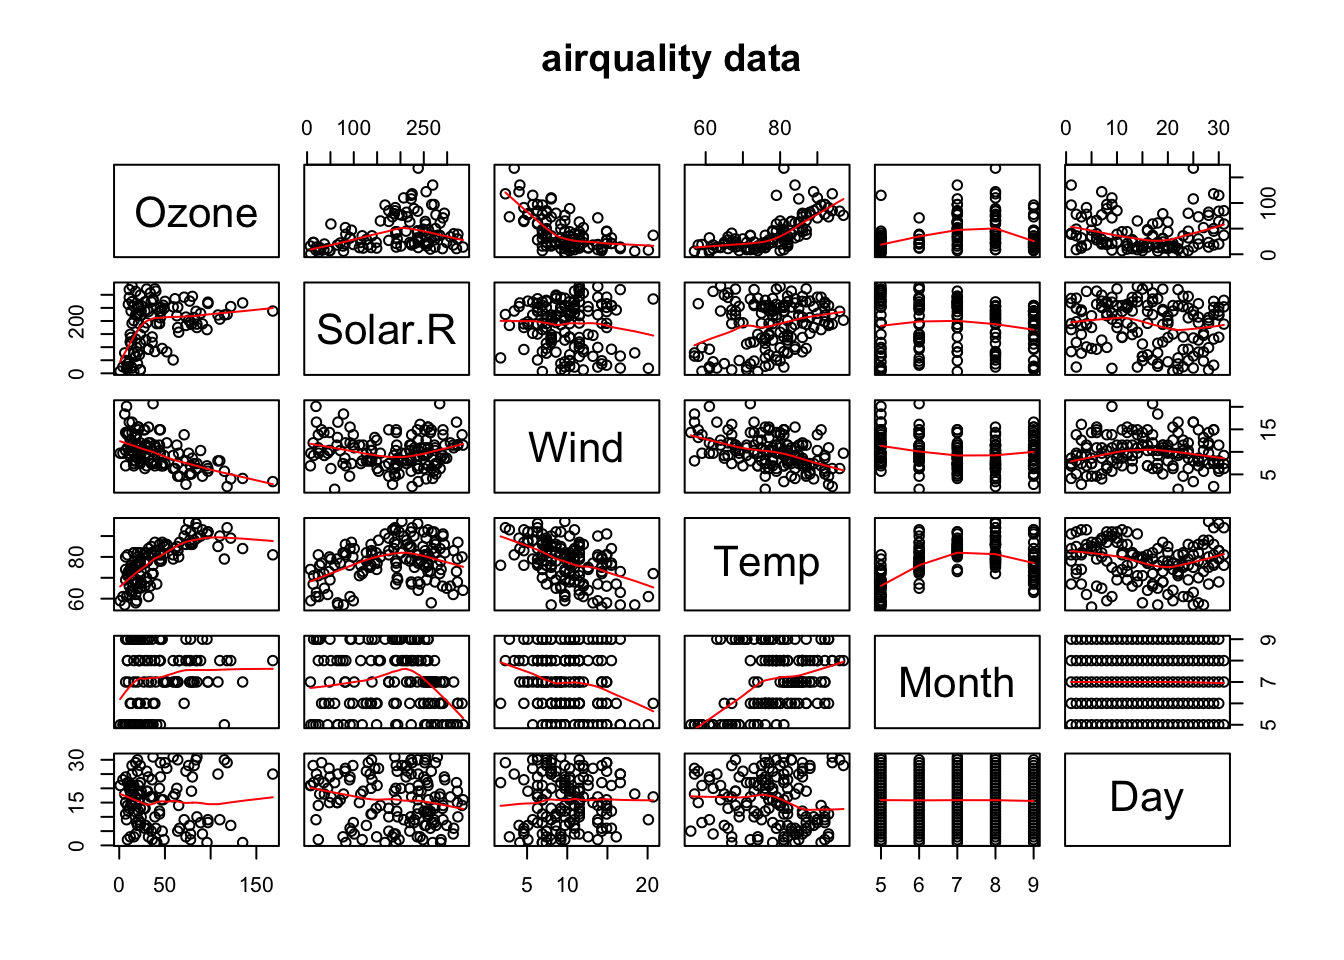
\includegraphics{bookdown-demo_files/figure-latex/unnamed-chunk-58-1.pdf}

\begin{Shaded}
\begin{Highlighting}[]
\NormalTok{ok <-}\StringTok{ }\KeywordTok{complete.cases}\NormalTok{(airquality)}
\NormalTok{airquality[ok,]}
\end{Highlighting}
\end{Shaded}

\section{Trabajando con data frames}\label{trabajando-con-data-frames-1}

\begin{itemize}
\tightlist
\item
  Los data frame se utilizand para guardas tablas de datos. Contiene
  elementos de la misma longitud.
\end{itemize}

\begin{Shaded}
\begin{Highlighting}[]
\NormalTok{mtcars}
\NormalTok{?mtcars       }\CommentTok{# help(mtcars)}
\end{Highlighting}
\end{Shaded}

\begin{itemize}
\tightlist
\item
  Observemos las primeras filas
\end{itemize}

\begin{Shaded}
\begin{Highlighting}[]
\KeywordTok{head}\NormalTok{(mtcars)}
\end{Highlighting}
\end{Shaded}

\begin{verbatim}
##                    mpg cyl disp  hp drat    wt  qsec vs am gear carb
## Mazda RX4         21.0   6  160 110 3.90 2.620 16.46  0  1    4    4
## Mazda RX4 Wag     21.0   6  160 110 3.90 2.875 17.02  0  1    4    4
## Datsun 710        22.8   4  108  93 3.85 2.320 18.61  1  1    4    1
## Hornet 4 Drive    21.4   6  258 110 3.08 3.215 19.44  1  0    3    1
## Hornet Sportabout 18.7   8  360 175 3.15 3.440 17.02  0  0    3    2
## Valiant           18.1   6  225 105 2.76 3.460 20.22  1  0    3    1
\end{verbatim}

\begin{itemize}
\tightlist
\item
  Estructura de un data frame
\end{itemize}

\begin{Shaded}
\begin{Highlighting}[]
\KeywordTok{str}\NormalTok{(mtcars) }\CommentTok{# visualiza la estructura del marco de datos}
\end{Highlighting}
\end{Shaded}

\begin{verbatim}
## 'data.frame':    32 obs. of  11 variables:
##  $ mpg : num  21 21 22.8 21.4 18.7 18.1 14.3 24.4 22.8 19.2 ...
##  $ cyl : num  6 6 4 6 8 6 8 4 4 6 ...
##  $ disp: num  160 160 108 258 360 ...
##  $ hp  : num  110 110 93 110 175 105 245 62 95 123 ...
##  $ drat: num  3.9 3.9 3.85 3.08 3.15 2.76 3.21 3.69 3.92 3.92 ...
##  $ wt  : num  2.62 2.88 2.32 3.21 3.44 ...
##  $ qsec: num  16.5 17 18.6 19.4 17 ...
##  $ vs  : num  0 0 1 1 0 1 0 1 1 1 ...
##  $ am  : num  1 1 1 0 0 0 0 0 0 0 ...
##  $ gear: num  4 4 4 3 3 3 3 4 4 4 ...
##  $ carb: num  4 4 1 1 2 1 4 2 2 4 ...
\end{verbatim}

\begin{itemize}
\tightlist
\item
  Select a car model:
\end{itemize}

\begin{Shaded}
\begin{Highlighting}[]
\NormalTok{mtcars[}\StringTok{"Mazda RX4"}\NormalTok{,] }\CommentTok{# usando nombres de las filas y las columnas}
\end{Highlighting}
\end{Shaded}

\begin{verbatim}
##           mpg cyl disp  hp drat   wt  qsec vs am gear carb
## Mazda RX4  21   6  160 110  3.9 2.62 16.46  0  1    4    4
\end{verbatim}

\begin{Shaded}
\begin{Highlighting}[]
\NormalTok{mtcars[}\KeywordTok{c}\NormalTok{(}\StringTok{"Datsun 710"}\NormalTok{, }\StringTok{"Camaro Z28"}\NormalTok{),] }
\end{Highlighting}
\end{Shaded}

\begin{verbatim}
##             mpg cyl disp  hp drat   wt  qsec vs am gear carb
## Datsun 710 22.8   4  108  93 3.85 2.32 18.61  1  1    4    1
## Camaro Z28 13.3   8  350 245 3.73 3.84 15.41  0  0    3    4
\end{verbatim}

\begin{itemize}
\tightlist
\item
  O variables concretas
\end{itemize}

\begin{Shaded}
\begin{Highlighting}[]
\NormalTok{mtcars[,}\KeywordTok{c}\NormalTok{(}\StringTok{"mpg"}\NormalTok{,}\StringTok{"am"}\NormalTok{)]}
\end{Highlighting}
\end{Shaded}

\begin{verbatim}
##                      mpg am
## Mazda RX4           21.0  1
## Mazda RX4 Wag       21.0  1
## Datsun 710          22.8  1
## Hornet 4 Drive      21.4  0
## Hornet Sportabout   18.7  0
## Valiant             18.1  0
## Duster 360          14.3  0
## Merc 240D           24.4  0
## Merc 230            22.8  0
## Merc 280            19.2  0
## Merc 280C           17.8  0
## Merc 450SE          16.4  0
## Merc 450SL          17.3  0
## Merc 450SLC         15.2  0
## Cadillac Fleetwood  10.4  0
## Lincoln Continental 10.4  0
## Chrysler Imperial   14.7  0
## Fiat 128            32.4  1
## Honda Civic         30.4  1
## Toyota Corolla      33.9  1
## Toyota Corona       21.5  0
## Dodge Challenger    15.5  0
## AMC Javelin         15.2  0
## Camaro Z28          13.3  0
## Pontiac Firebird    19.2  0
## Fiat X1-9           27.3  1
## Porsche 914-2       26.0  1
## Lotus Europa        30.4  1
## Ford Pantera L      15.8  1
## Ferrari Dino        19.7  1
## Maserati Bora       15.0  1
## Volvo 142E          21.4  1
\end{verbatim}

\begin{Shaded}
\begin{Highlighting}[]
\KeywordTok{library}\NormalTok{(psych)}
\KeywordTok{describe}\NormalTok{(mtcars)}
\end{Highlighting}
\end{Shaded}

\begin{verbatim}
##                                                    25%        50% 
##  352.00000   39.60853   84.20792    0.00000    2.42875    4.00000 
##        75%                       
##   18.97500  472.00000 -341.00000
\end{verbatim}

\chapter{\texorpdfstring{Análisis de datos básico en
\texttt{R}}{Análisis de datos básico en R}}\label{analisis-de-datos-basico-en-r}

\section{Gráficos sencillos}\label{graficos-sencillos}

\begin{itemize}
\tightlist
\item
  Scatterplot
\end{itemize}

\begin{Shaded}
\begin{Highlighting}[]
\KeywordTok{attach}\NormalTok{(mtcars)}
\end{Highlighting}
\end{Shaded}

\begin{verbatim}
## The following object is masked from package:ggplot2:
## 
##     mpg
\end{verbatim}

\begin{verbatim}
## The following objects are masked from mtcars (pos = 21):
## 
##     am, carb, cyl, disp, drat, gear, hp, mpg, qsec, vs, wt
\end{verbatim}

\begin{Shaded}
\begin{Highlighting}[]
\KeywordTok{plot}\NormalTok{(wt, mpg, }\DataTypeTok{main=}\StringTok{"Scatterplot Example"}\NormalTok{,}
   \DataTypeTok{xlab=}\StringTok{"Car Weight "}\NormalTok{, }\DataTypeTok{ylab=}\StringTok{"Miles Per Gallon "}\NormalTok{, }\DataTypeTok{pch=}\DecValTok{19}\NormalTok{) }
\end{Highlighting}
\end{Shaded}

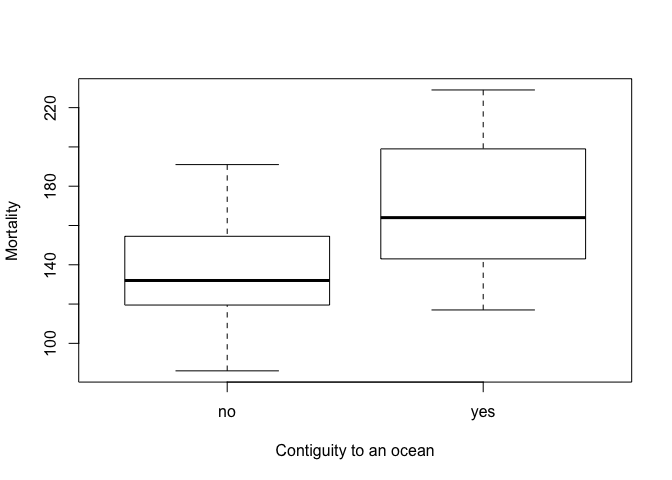
\includegraphics{bookdown-demo_files/figure-latex/unnamed-chunk-65-1.pdf}

\begin{itemize}
\tightlist
\item
  Matriz scatterplot
\end{itemize}

\begin{Shaded}
\begin{Highlighting}[]
\KeywordTok{pairs}\NormalTok{(}\OperatorTok{~}\NormalTok{mpg}\OperatorTok{+}\NormalTok{disp}\OperatorTok{+}\NormalTok{drat}\OperatorTok{+}\NormalTok{wt,}\DataTypeTok{data=}\NormalTok{mtcars,}
   \DataTypeTok{main=}\StringTok{"Simple Scatterplot Matrix"}\NormalTok{)}
\end{Highlighting}
\end{Shaded}

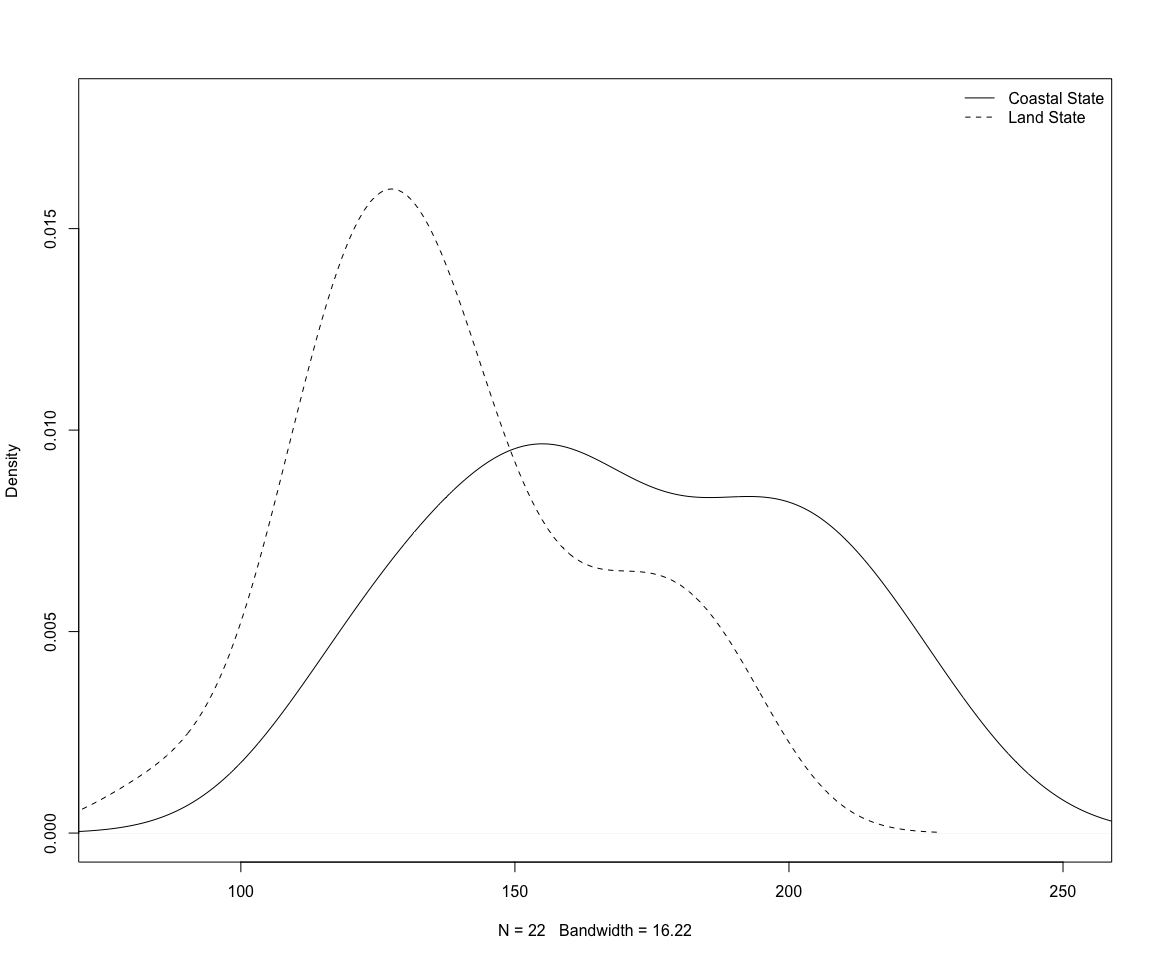
\includegraphics{bookdown-demo_files/figure-latex/unnamed-chunk-66-1.pdf}

\begin{itemize}
\tightlist
\item
  Barplot o diagrama de barras
\end{itemize}

\begin{Shaded}
\begin{Highlighting}[]
\NormalTok{tab <-}\StringTok{ }\KeywordTok{table}\NormalTok{(mtcars[,}\KeywordTok{c}\NormalTok{(}\StringTok{"cyl"}\NormalTok{)])}
\KeywordTok{barplot}\NormalTok{(tab)}
\end{Highlighting}
\end{Shaded}

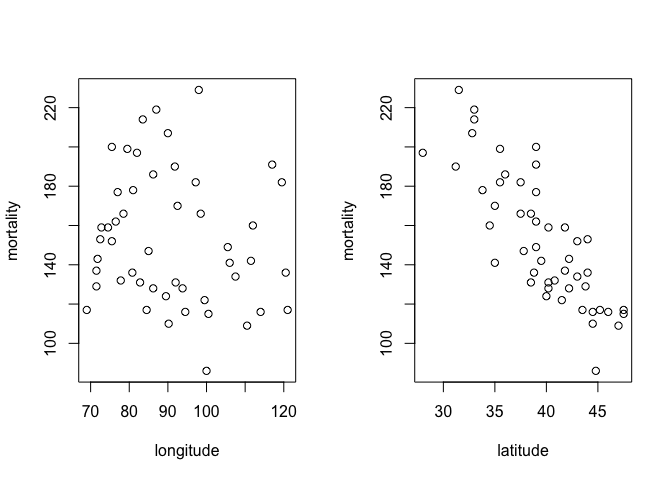
\includegraphics{bookdown-demo_files/figure-latex/unnamed-chunk-67-1.pdf}

\begin{itemize}
\tightlist
\item
  Piechart o diagrama de tarta
\end{itemize}

\begin{Shaded}
\begin{Highlighting}[]
\KeywordTok{pie}\NormalTok{(tab)}
\end{Highlighting}
\end{Shaded}

\begin{center}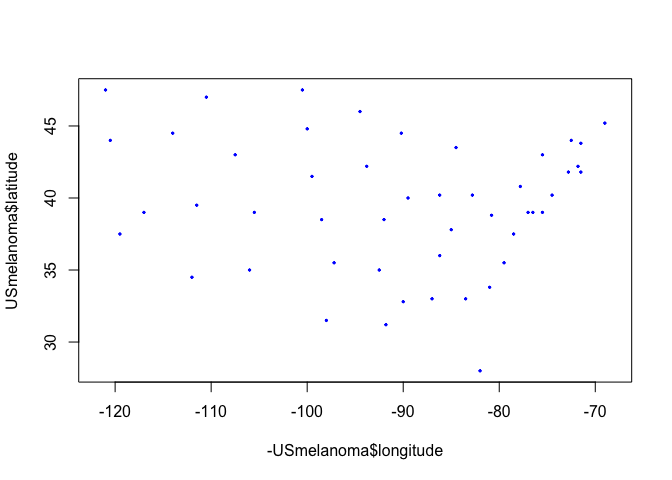
\includegraphics{bookdown-demo_files/figure-latex/unnamed-chunk-68-1} \end{center}

\textbf{Ejercicio:}

\begin{enumerate}
\def\labelenumi{\arabic{enumi}.}
\tightlist
\item
  El \texttt{data.frame} \texttt{VADeaths} contiene las tasas de
  mortalidad por cada 1000 habitantes en Virginia (EEUU) en 1940
\end{enumerate}

\begin{itemize}
\tightlist
\item
  Las tasas de mortalidad se miden cada 1000 habitantes por año. Se
  encuentran clasificadas por grupo de edad (filas) y grupo de población
  (columnas). Los grupos de edad son: 50-54, 55-59, 60-64, 65-69, 70-74
  y los grupos de población: \texttt{Rural/Male}, \texttt{Rural/Female},
  \texttt{Urban/Male} and \texttt{Urban/Female}.
\end{itemize}

\begin{Shaded}
\begin{Highlighting}[]
\KeywordTok{data}\NormalTok{(VADeaths)}
\NormalTok{VADeaths}
\end{Highlighting}
\end{Shaded}

\begin{verbatim}
##       Rural Male Rural Female Urban Male Urban Female
## 50-54       11.7          8.7       15.4          8.4
## 55-59       18.1         11.7       24.3         13.6
## 60-64       26.9         20.3       37.0         19.3
## 65-69       41.0         30.9       54.6         35.1
## 70-74       66.0         54.3       71.1         50.0
\end{verbatim}

\begin{itemize}
\item
  Calcula la media para cada grupo de edad.

  \begin{itemize}
  \tightlist
  \item
    \textbf{Result:}
  \end{itemize}
\end{itemize}

\begin{verbatim}
##  50-54  55-59  60-64  65-69  70-74 
## 11.050 16.925 25.875 40.400 60.350
\end{verbatim}

\begin{itemize}
\item
  Calcula la media para cada grupo de población.

  \begin{itemize}
  \tightlist
  \item
    \textbf{Resultado:}
  \end{itemize}
\end{itemize}

\begin{verbatim}
##   Rural Male Rural Female   Urban Male Urban Female 
##        32.74        25.18        40.48        25.28
\end{verbatim}

\begin{enumerate}
\def\labelenumi{\arabic{enumi}.}
\setcounter{enumi}{1}
\tightlist
\item
  El \texttt{data.frame} \texttt{rainforest} contiene diferentes
  variables de \texttt{species}
\end{enumerate}

\begin{Shaded}
\begin{Highlighting}[]
\KeywordTok{library}\NormalTok{(DAAG)}
\NormalTok{rainforest}
\NormalTok{?rainforest}
\KeywordTok{names}\NormalTok{(rainforest)}
\end{Highlighting}
\end{Shaded}

\begin{itemize}
\item
  Crear una tabla de conteos para cada \texttt{species} y realiza un
  gráfico descriptivo.

  \begin{itemize}
  \tightlist
  \item
    \textbf{Resultado:}
  \end{itemize}
\end{itemize}

\begin{verbatim}
## 
## Acacia mabellae      C. fraseri  Acmena smithii   B. myrtifolia 
##              16              12              26              11
\end{verbatim}

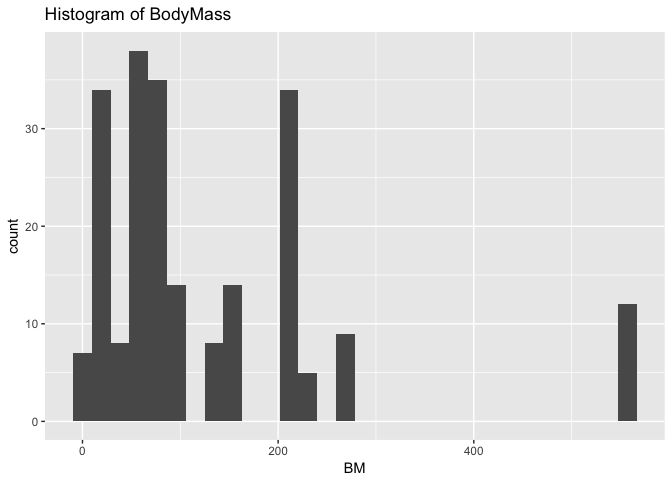
\includegraphics{bookdown-demo_files/figure-latex/unnamed-chunk-73-1.pdf}

\begin{enumerate}
\def\labelenumi{\arabic{enumi}.}
\setcounter{enumi}{2}
\tightlist
\item
  El \texttt{data.frame} \texttt{Acmena} est? creado a partir de
  \texttt{rainforest} mediante la función \texttt{subset}.
\end{enumerate}

\begin{itemize}
\tightlist
\item
  Realiza un gráfico que relacione la biomasa de la madera
  (\texttt{wood}) y el di?metro a la altura del pecho (\texttt{dbh}).
  Utiliza tambi?n la escala logarítmica.
\end{itemize}

\begin{Shaded}
\begin{Highlighting}[]
\NormalTok{Acmena <-}\StringTok{ }\KeywordTok{subset}\NormalTok{(rainforest, species }\OperatorTok{==}\StringTok{ "Acmena smithii"}\NormalTok{)}
\end{Highlighting}
\end{Shaded}

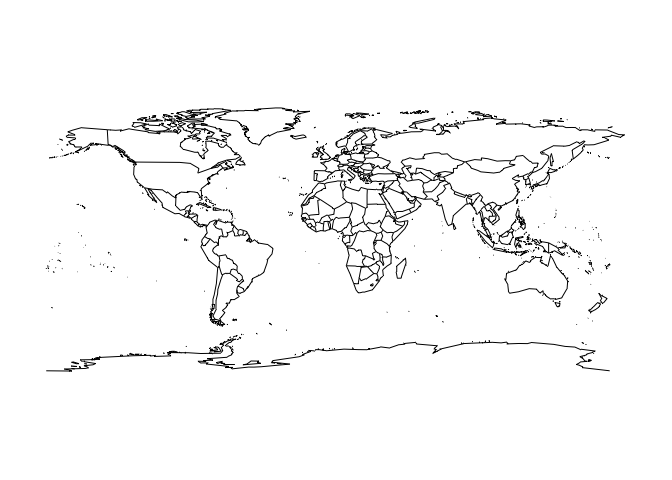
\includegraphics{bookdown-demo_files/figure-latex/unnamed-chunk-75-1.pdf}

\begin{itemize}
\tightlist
\item
  Calcula un histograma de la variable \texttt{dbh} mediante la función
  \texttt{hist}
\end{itemize}

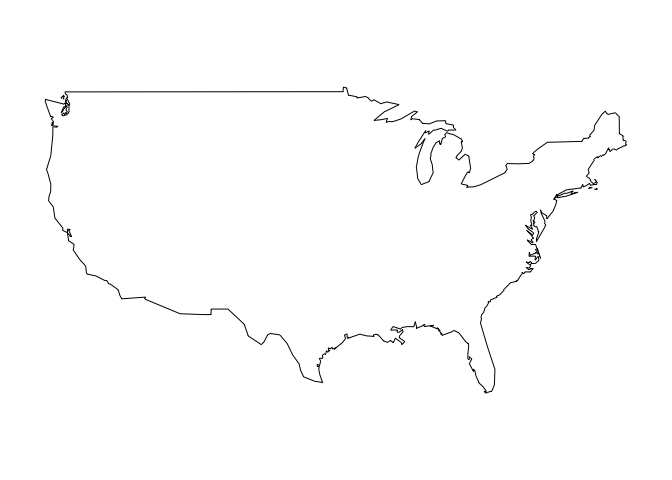
\includegraphics{bookdown-demo_files/figure-latex/unnamed-chunk-76-1.pdf}

\begin{enumerate}
\def\labelenumi{\arabic{enumi}.}
\setcounter{enumi}{3}
\item
  Crea un vector de n?meros enteros positivos impares the longitud 100 y
  calcula los valores entre 60 y 80.

  \begin{itemize}
  \tightlist
  \item
    \textbf{Result:}
  \end{itemize}
\end{enumerate}

\begin{verbatim}
##  [1] 61 63 65 67 69 71 73 75 77 79
\end{verbatim}

\begin{itemize}
\tightlist
\item
  \href{http://idaejin.github.io/bcam-courses/rbasics/rbasics_sol.R}{Soluciones
  aquí}
\end{itemize}

\begin{center}\rule{0.5\linewidth}{\linethickness}\end{center}

\section{Scatterplots}\label{scatterplots}

\begin{Shaded}
\begin{Highlighting}[]
\KeywordTok{library}\NormalTok{(MASS)}
\KeywordTok{data}\NormalTok{(}\StringTok{"mammals"}\NormalTok{)}
\NormalTok{?mammals}
\KeywordTok{head}\NormalTok{(mammals)}
\end{Highlighting}
\end{Shaded}

\begin{verbatim}
##                    body brain
## Arctic fox        3.385  44.5
## Owl monkey        0.480  15.5
## Mountain beaver   1.350   8.1
## Cow             465.000 423.0
## Grey wolf        36.330 119.5
## Goat             27.660 115.0
\end{verbatim}

\begin{Shaded}
\begin{Highlighting}[]
\KeywordTok{attach}\NormalTok{(mammals)}
\NormalTok{species <-}\StringTok{ }\KeywordTok{row.names}\NormalTok{(mammals)}
\NormalTok{x <-}\StringTok{ }\NormalTok{body}
\NormalTok{y <-}\StringTok{ }\NormalTok{brain}
\end{Highlighting}
\end{Shaded}

\begin{Shaded}
\begin{Highlighting}[]
\KeywordTok{library}\NormalTok{(calibrate)}
\CommentTok{# scatterplot}
\KeywordTok{plot}\NormalTok{(x,y, }\DataTypeTok{xlab =} \StringTok{"body weight in kgr"}\NormalTok{, }\DataTypeTok{ylab =} \StringTok{"brain weight in gr"}\NormalTok{, }
     \DataTypeTok{main=}\StringTok{"Body vs Brain weight }\CharTok{\textbackslash{}n}\StringTok{ for 62 Species of Land Mammals"}\NormalTok{,}\DataTypeTok{xlim=}\KeywordTok{c}\NormalTok{(}\DecValTok{0}\NormalTok{,}\DecValTok{8500}\NormalTok{))}
\KeywordTok{textxy}\NormalTok{(x,y,}\DataTypeTok{labs=}\NormalTok{species,}\DataTypeTok{col =} \StringTok{"blue"}\NormalTok{,}\DataTypeTok{cex=}\FloatTok{0.85}\NormalTok{) }
\end{Highlighting}
\end{Shaded}

\begin{center}\includegraphics{bookdown-demo_files/figure-latex/unnamed-chunk-79-1} \end{center}

Identificar un punto en el scatterplot

\begin{Shaded}
\begin{Highlighting}[]
\KeywordTok{identify}\NormalTok{(x,y,species)}
\end{Highlighting}
\end{Shaded}

En escala logarítmica

\begin{Shaded}
\begin{Highlighting}[]
\KeywordTok{plot}\NormalTok{(}\KeywordTok{log}\NormalTok{(x),}\KeywordTok{log}\NormalTok{(y), }\DataTypeTok{xlab =} \StringTok{"log body weight in kgr"}\NormalTok{, }\DataTypeTok{ylab =} \StringTok{"log brain weight in gr"}\NormalTok{, }
     \DataTypeTok{main=}\StringTok{"log Body vs log Brain weight }\CharTok{\textbackslash{}n}\StringTok{ for 62 Species of Land Mammals"}\NormalTok{)}
\KeywordTok{textxy}\NormalTok{(}\KeywordTok{log}\NormalTok{(x),}\KeywordTok{log}\NormalTok{(y),}\DataTypeTok{labs=}\NormalTok{species,}\DataTypeTok{col =} \StringTok{"blue"}\NormalTok{,}\DataTypeTok{cex=}\FloatTok{0.85}\NormalTok{) }
\end{Highlighting}
\end{Shaded}

\begin{center}\includegraphics{bookdown-demo_files/figure-latex/unnamed-chunk-81-1} \end{center}

Identificar un punto en la escala logarítmica

\begin{Shaded}
\begin{Highlighting}[]
\KeywordTok{identify}\NormalTok{(}\KeywordTok{log}\NormalTok{(x),}\KeywordTok{log}\NormalTok{(y),species)}
\end{Highlighting}
\end{Shaded}

\section{más opciones gráficas}\label{mas-opciones-graficas}

\textbf{Varios conjuntos de datos en un sólo gráfico}

Una vez realizado un \texttt{plot}, el comando \texttt{points} permite
aadir nuevas observaciones.

\begin{Shaded}
\begin{Highlighting}[]
\KeywordTok{set.seed}\NormalTok{(}\DecValTok{1234}\NormalTok{)}
\NormalTok{ x <-}\StringTok{ }\KeywordTok{rnorm}\NormalTok{(}\DecValTok{10}\NormalTok{,}\DataTypeTok{sd=}\DecValTok{5}\NormalTok{,}\DataTypeTok{mean=}\DecValTok{20}\NormalTok{)}
\NormalTok{ y <-}\StringTok{ }\FloatTok{2.5}\OperatorTok{*}\NormalTok{x }\OperatorTok{-}\StringTok{ }\FloatTok{1.0} \OperatorTok{+}\StringTok{ }\KeywordTok{rnorm}\NormalTok{(}\DecValTok{10}\NormalTok{,}\DataTypeTok{sd=}\DecValTok{9}\NormalTok{,}\DataTypeTok{mean=}\DecValTok{0}\NormalTok{)}
 \KeywordTok{cor}\NormalTok{(x,y)}
\end{Highlighting}
\end{Shaded}

\begin{verbatim}
## [1] 0.7512194
\end{verbatim}

\begin{Shaded}
\begin{Highlighting}[]
 \KeywordTok{plot}\NormalTok{(x,y,}\DataTypeTok{xlab=}\StringTok{"Independent"}\NormalTok{,}\DataTypeTok{ylab=}\StringTok{"Dependent"}\NormalTok{,}\DataTypeTok{main=}\StringTok{"Random plot"}\NormalTok{)}
\NormalTok{ x1 <-}\StringTok{ }\KeywordTok{runif}\NormalTok{(}\DecValTok{8}\NormalTok{,}\DecValTok{15}\NormalTok{,}\DecValTok{25}\NormalTok{)}
\NormalTok{ y1 <-}\StringTok{ }\FloatTok{2.5}\OperatorTok{*}\NormalTok{x1 }\OperatorTok{-}\StringTok{ }\FloatTok{1.0} \OperatorTok{+}\StringTok{ }\KeywordTok{runif}\NormalTok{(}\DecValTok{8}\NormalTok{,}\OperatorTok{-}\DecValTok{6}\NormalTok{,}\DecValTok{6}\NormalTok{)}
 \KeywordTok{points}\NormalTok{(x1,y1,}\DataTypeTok{col=}\DecValTok{2}\NormalTok{)}
\end{Highlighting}
\end{Shaded}

\includegraphics{bookdown-demo_files/figure-latex/unnamed-chunk-83-1.pdf}

con la leyenda

\begin{Shaded}
\begin{Highlighting}[]
\KeywordTok{set.seed}\NormalTok{(}\DecValTok{1234}\NormalTok{)}
\NormalTok{x2 <-}\StringTok{ }\KeywordTok{runif}\NormalTok{(}\DecValTok{8}\NormalTok{,}\DecValTok{15}\NormalTok{,}\DecValTok{25}\NormalTok{)}
\NormalTok{y2 <-}\StringTok{ }\FloatTok{2.5}\OperatorTok{*}\NormalTok{x2 }\OperatorTok{-}\StringTok{ }\FloatTok{1.0} \OperatorTok{+}\StringTok{ }\KeywordTok{runif}\NormalTok{(}\DecValTok{8}\NormalTok{,}\OperatorTok{-}\DecValTok{6}\NormalTok{,}\DecValTok{6}\NormalTok{)}
 \KeywordTok{plot}\NormalTok{(x,y,}\DataTypeTok{xlab=}\StringTok{"Independent"}\NormalTok{,}\DataTypeTok{ylab=}\StringTok{"Dependent"}\NormalTok{,}\DataTypeTok{main=}\StringTok{"Random plot"}\NormalTok{)}
 \KeywordTok{points}\NormalTok{(x1,y1,}\DataTypeTok{col=}\DecValTok{2}\NormalTok{,}\DataTypeTok{pch=}\DecValTok{3}\NormalTok{)}
 \KeywordTok{points}\NormalTok{(x2,y2,}\DataTypeTok{col=}\DecValTok{4}\NormalTok{,}\DataTypeTok{pch=}\DecValTok{5}\NormalTok{)}
 \KeywordTok{legend}\NormalTok{(}\StringTok{"topleft"}\NormalTok{,}\KeywordTok{c}\NormalTok{(}\StringTok{"Original"}\NormalTok{,}\StringTok{"one"}\NormalTok{,}\StringTok{"two"}\NormalTok{),}\DataTypeTok{col=}\KeywordTok{c}\NormalTok{(}\DecValTok{1}\NormalTok{,}\DecValTok{2}\NormalTok{,}\DecValTok{4}\NormalTok{),}\DataTypeTok{pch=}\KeywordTok{c}\NormalTok{(}\DecValTok{1}\NormalTok{,}\DecValTok{3}\NormalTok{,}\DecValTok{5}\NormalTok{))}
\end{Highlighting}
\end{Shaded}

\includegraphics{bookdown-demo_files/figure-latex/unnamed-chunk-84-1.pdf}

\textbf{Varios gráficos en un sola imagen}

\begin{Shaded}
\begin{Highlighting}[]
\KeywordTok{set.seed}\NormalTok{(}\DecValTok{1234}\NormalTok{)}
 \KeywordTok{par}\NormalTok{(}\DataTypeTok{mfrow=}\KeywordTok{c}\NormalTok{(}\DecValTok{2}\NormalTok{,}\DecValTok{3}\NormalTok{))}
 \KeywordTok{boxplot}\NormalTok{(}\KeywordTok{rnorm}\NormalTok{(}\DecValTok{100}\NormalTok{),}\DataTypeTok{main=}\StringTok{"first plot"}\NormalTok{)}
 \KeywordTok{boxplot}\NormalTok{(}\KeywordTok{rgamma}\NormalTok{(}\DecValTok{100}\NormalTok{,}\DecValTok{2}\NormalTok{),}\DataTypeTok{main=}\StringTok{"second plot"}\NormalTok{, }\DataTypeTok{horizontal=}\OtherTok{TRUE}\NormalTok{,}\DataTypeTok{col=}\StringTok{"bisque"}\NormalTok{)}
 \KeywordTok{plot}\NormalTok{(}\KeywordTok{rnorm}\NormalTok{(}\DecValTok{100}\NormalTok{),}\DataTypeTok{xlab=}\StringTok{"third plot"}\NormalTok{,}
      \DataTypeTok{ylab=}\StringTok{"y-label"}\NormalTok{,}\DataTypeTok{main=}\StringTok{"x-label"}\NormalTok{)}
 \KeywordTok{hist}\NormalTok{(}\KeywordTok{rnorm}\NormalTok{(}\DecValTok{100}\NormalTok{),}\DataTypeTok{main=}\StringTok{"fourth plot"}\NormalTok{,}\DataTypeTok{col=}\StringTok{"lightgrey"}\NormalTok{)}
 \KeywordTok{hist}\NormalTok{(}\KeywordTok{rexp}\NormalTok{(}\DecValTok{100}\NormalTok{),}\DataTypeTok{main=}\StringTok{"fifth plot"}\NormalTok{,}\DataTypeTok{col=}\StringTok{"blue"}\NormalTok{)}
 \KeywordTok{plot}\NormalTok{(}\KeywordTok{rnorm}\NormalTok{(}\DecValTok{100}\NormalTok{),}\KeywordTok{rexp}\NormalTok{(}\DecValTok{100}\NormalTok{),}\DataTypeTok{main=}\StringTok{"sixth plot"}\NormalTok{)}
\end{Highlighting}
\end{Shaded}

\includegraphics{bookdown-demo_files/figure-latex/unnamed-chunk-85-1.pdf}

\textbf{Relaciones entre variables}

\begin{Shaded}
\begin{Highlighting}[]
\NormalTok{uData <-}\StringTok{ }\KeywordTok{rnorm}\NormalTok{(}\DecValTok{20}\NormalTok{)}
\NormalTok{vData <-}\StringTok{ }\KeywordTok{rnorm}\NormalTok{(}\DecValTok{20}\NormalTok{,}\DataTypeTok{mean=}\DecValTok{5}\NormalTok{)}
\NormalTok{wData <-}\StringTok{ }\NormalTok{uData }\OperatorTok{+}\StringTok{ }\DecValTok{2}\OperatorTok{*}\NormalTok{vData }\OperatorTok{+}\StringTok{ }\KeywordTok{rnorm}\NormalTok{(}\DecValTok{20}\NormalTok{,}\DataTypeTok{sd=}\FloatTok{0.5}\NormalTok{)}
\NormalTok{xData <-}\StringTok{ }\OperatorTok{-}\DecValTok{2}\OperatorTok{*}\NormalTok{uData}\OperatorTok{+}\KeywordTok{rnorm}\NormalTok{(}\DecValTok{20}\NormalTok{,}\DataTypeTok{sd=}\FloatTok{0.1}\NormalTok{)}
\NormalTok{yData <-}\StringTok{  }\DecValTok{3}\OperatorTok{*}\NormalTok{vData}\OperatorTok{+}\KeywordTok{rnorm}\NormalTok{(}\DecValTok{20}\NormalTok{,}\DataTypeTok{sd=}\FloatTok{2.5}\NormalTok{)}
\NormalTok{d <-}\StringTok{ }\KeywordTok{data.frame}\NormalTok{(}\DataTypeTok{u=}\NormalTok{uData,}\DataTypeTok{v=}\NormalTok{vData,}\DataTypeTok{w=}\NormalTok{wData,}\DataTypeTok{x=}\NormalTok{xData,}\DataTypeTok{y=}\NormalTok{yData)}
\KeywordTok{pairs}\NormalTok{(d)}
\end{Highlighting}
\end{Shaded}

\includegraphics{bookdown-demo_files/figure-latex/unnamed-chunk-86-1.pdf}

\textbf{Gráfico de correlaciones}

La función \texttt{corrplot} de la librer?a \texttt{corrplot} permite
visualizar una matriz de correlaciones calculada mediante la función
\texttt{cor}

\begin{Shaded}
\begin{Highlighting}[]
\KeywordTok{library}\NormalTok{(corrplot)}
\NormalTok{M <-}\StringTok{ }\KeywordTok{cor}\NormalTok{(d)}
\KeywordTok{corrplot}\NormalTok{(M, }\DataTypeTok{method=}\StringTok{"circle"}\NormalTok{,}\DataTypeTok{type=}\StringTok{"upper"}\NormalTok{)}
\end{Highlighting}
\end{Shaded}

\includegraphics{bookdown-demo_files/figure-latex/unnamed-chunk-87-1.pdf}

\textbf{Gráficos de superficies: \texttt{image}, \texttt{contour} y
\texttt{persp}}

\begin{Shaded}
\begin{Highlighting}[]
\NormalTok{x <-}\StringTok{ }\KeywordTok{seq}\NormalTok{(}\DecValTok{0}\NormalTok{,}\DecValTok{2}\OperatorTok{*}\NormalTok{pi,}\DataTypeTok{by=}\NormalTok{pi}\OperatorTok{/}\DecValTok{50}\NormalTok{)}
\NormalTok{y <-}\StringTok{ }\NormalTok{x}
\NormalTok{xg <-}\StringTok{ }\NormalTok{(x}\OperatorTok{*}\DecValTok{0}\OperatorTok{+}\DecValTok{1}\NormalTok{) }\OperatorTok\StringTok{ }\KeywordTok{t}\NormalTok{(y)}
\NormalTok{yg <-}\StringTok{ }\NormalTok{(x) }\OperatorTok\StringTok{ }\KeywordTok{t}\NormalTok{(y}\OperatorTok{*}\DecValTok{0}\OperatorTok{+}\DecValTok{1}\NormalTok{)}
\NormalTok{f <-}\StringTok{ }\KeywordTok{sin}\NormalTok{(xg}\OperatorTok{*}\NormalTok{yg)}

\KeywordTok{par}\NormalTok{(}\DataTypeTok{mfrow=}\KeywordTok{c}\NormalTok{(}\DecValTok{2}\NormalTok{,}\DecValTok{2}\NormalTok{))}
\KeywordTok{image}\NormalTok{(x,y,f)}
\KeywordTok{contour}\NormalTok{(x,y,f)}
\KeywordTok{contour}\NormalTok{(x,y,f,}\DataTypeTok{nlevels=}\DecValTok{4}\NormalTok{)}
\KeywordTok{image}\NormalTok{(x,y,f,}\DataTypeTok{col=}\KeywordTok{grey.colors}\NormalTok{(}\DecValTok{100}\NormalTok{))}
\KeywordTok{contour}\NormalTok{(x,y,f,}\DataTypeTok{nlevels=}\DecValTok{4}\NormalTok{,}\DataTypeTok{add=}\OtherTok{TRUE}\NormalTok{,}\DataTypeTok{col=}\StringTok{"red"}\NormalTok{)}
\end{Highlighting}
\end{Shaded}

\includegraphics{bookdown-demo_files/figure-latex/unnamed-chunk-88-1.pdf}

Podemos utilizar la función \texttt{persp}

\begin{Shaded}
\begin{Highlighting}[]
\KeywordTok{persp}\NormalTok{(x,y,f,}\DataTypeTok{theta=}\OperatorTok{-}\DecValTok{30}\NormalTok{,}\DataTypeTok{phi=}\DecValTok{55}\NormalTok{,}\DataTypeTok{col=}\StringTok{"lightgrey"}\NormalTok{,}\DataTypeTok{shade=}\NormalTok{.}\DecValTok{01}\NormalTok{)}
\end{Highlighting}
\end{Shaded}

\begin{center}\includegraphics{bookdown-demo_files/figure-latex/unnamed-chunk-89-1} \end{center}

o representar im?genes

\begin{Shaded}
\begin{Highlighting}[]
\KeywordTok{library}\NormalTok{(fields)}
\KeywordTok{data}\NormalTok{(lennon)}
\KeywordTok{image}\NormalTok{(lennon,}\DataTypeTok{col=}\KeywordTok{grey}\NormalTok{(}\KeywordTok{seq}\NormalTok{(}\DecValTok{0}\NormalTok{,}\DecValTok{1}\NormalTok{,}\DataTypeTok{l=}\DecValTok{256}\NormalTok{)))}
\end{Highlighting}
\end{Shaded}

\includegraphics{bookdown-demo_files/figure-latex/unnamed-chunk-90-1.pdf}

\section{Tablas de clasificación cruzada o de
contigencia}\label{tablas-de-clasificacion-cruzada-o-de-contigencia}

\begin{Shaded}
\begin{Highlighting}[]
\KeywordTok{library}\NormalTok{(MASS)}
\KeywordTok{data}\NormalTok{(quine)}
\KeywordTok{head}\NormalTok{(quine)}
\end{Highlighting}
\end{Shaded}

\begin{verbatim}
##   Eth Sex Age Lrn Days
## 1   A   M  F0  SL    2
## 2   A   M  F0  SL   11
## 3   A   M  F0  SL   14
## 4   A   M  F0  AL    5
## 5   A   M  F0  AL    5
## 6   A   M  F0  AL   13
\end{verbatim}

\begin{Shaded}
\begin{Highlighting}[]
\KeywordTok{attach}\NormalTok{(quine)}
\end{Highlighting}
\end{Shaded}

\begin{verbatim}
## The following objects are masked from quine (pos = 13):
## 
##     Age, Days, Eth, Lrn, Sex
\end{verbatim}

\begin{Shaded}
\begin{Highlighting}[]
\KeywordTok{table}\NormalTok{(Sex)}
\end{Highlighting}
\end{Shaded}

\begin{verbatim}
## Sex
##  F  M 
## 80 66
\end{verbatim}

\begin{Shaded}
\begin{Highlighting}[]
\KeywordTok{table}\NormalTok{(Sex,Age)}
\end{Highlighting}
\end{Shaded}

\begin{verbatim}
##    Age
## Sex F0 F1 F2 F3
##   F 10 32 19 19
##   M 17 14 21 14
\end{verbatim}

\begin{Shaded}
\begin{Highlighting}[]
\CommentTok{# or xtabs}
\KeywordTok{xtabs}\NormalTok{(}\OperatorTok{~}\NormalTok{Sex}\OperatorTok{+}\NormalTok{Age,}\DataTypeTok{data=}\NormalTok{quine)}
\end{Highlighting}
\end{Shaded}

\begin{verbatim}
##    Age
## Sex F0 F1 F2 F3
##   F 10 32 19 19
##   M 17 14 21 14
\end{verbatim}

\begin{Shaded}
\begin{Highlighting}[]
\KeywordTok{xtabs}\NormalTok{(}\OperatorTok{~}\NormalTok{Sex}\OperatorTok{+}\NormalTok{Age}\OperatorTok{+}\NormalTok{Eth,}\DataTypeTok{data=}\NormalTok{quine)}
\end{Highlighting}
\end{Shaded}

\begin{verbatim}
## , , Eth = A
## 
##    Age
## Sex F0 F1 F2 F3
##   F  5 15  9  9
##   M  8  5 11  7
## 
## , , Eth = N
## 
##    Age
## Sex F0 F1 F2 F3
##   F  5 17 10 10
##   M  9  9 10  7
\end{verbatim}

\section{cálculos sobre tablas de
contigencia}\label{calculos-sobre-tablas-de-contigencia}

\begin{Shaded}
\begin{Highlighting}[]
\KeywordTok{tapply}\NormalTok{(Days,Age,mean)}
\end{Highlighting}
\end{Shaded}

\begin{verbatim}
##       F0       F1       F2       F3 
## 14.85185 11.15217 21.05000 19.60606
\end{verbatim}

\begin{Shaded}
\begin{Highlighting}[]
\KeywordTok{tapply}\NormalTok{(Days,}\KeywordTok{list}\NormalTok{(Sex,Age),mean)}
\end{Highlighting}
\end{Shaded}

\begin{verbatim}
##         F0       F1       F2       F3
## F 18.70000 12.96875 18.42105 14.00000
## M 12.58824  7.00000 23.42857 27.21429
\end{verbatim}

\begin{Shaded}
\begin{Highlighting}[]
\KeywordTok{tapply}\NormalTok{(Days,}\KeywordTok{list}\NormalTok{(Sex,Age),}\ControlFlowTok{function}\NormalTok{(x) }\KeywordTok{sqrt}\NormalTok{(}\KeywordTok{var}\NormalTok{(x)}\OperatorTok{/}\KeywordTok{length}\NormalTok{(x)))}
\end{Highlighting}
\end{Shaded}

\begin{verbatim}
##         F0       F1       F2       F3
## F 4.208589 2.329892 5.299959 2.940939
## M 3.768151 1.418093 3.766122 4.569582
\end{verbatim}

\section{Datos cualitativos}\label{datos-cualitativos}

Supongamos unos datos cualquiera de las variables \texttt{treatment} y
\texttt{improvement} de pacientes a una enfermedad determinada.

\begin{Shaded}
\begin{Highlighting}[]
\NormalTok{treatment <-}\StringTok{ }\KeywordTok{factor}\NormalTok{(}\KeywordTok{rep}\NormalTok{(}\KeywordTok{c}\NormalTok{(}\DecValTok{1}\NormalTok{, }\DecValTok{2}\NormalTok{), }\KeywordTok{c}\NormalTok{(}\DecValTok{43}\NormalTok{, }\DecValTok{41}\NormalTok{)), }\DataTypeTok{levels =} \KeywordTok{c}\NormalTok{(}\DecValTok{1}\NormalTok{, }\DecValTok{2}\NormalTok{),}
                    \DataTypeTok{labels =} \KeywordTok{c}\NormalTok{(}\StringTok{"placebo"}\NormalTok{, }\StringTok{"treated"}\NormalTok{))}
\NormalTok{improved <-}\StringTok{ }\KeywordTok{factor}\NormalTok{(}\KeywordTok{rep}\NormalTok{(}\KeywordTok{c}\NormalTok{(}\DecValTok{1}\NormalTok{, }\DecValTok{2}\NormalTok{, }\DecValTok{3}\NormalTok{, }\DecValTok{1}\NormalTok{, }\DecValTok{2}\NormalTok{, }\DecValTok{3}\NormalTok{), }\KeywordTok{c}\NormalTok{(}\DecValTok{29}\NormalTok{, }\DecValTok{7}\NormalTok{, }\DecValTok{7}\NormalTok{, }\DecValTok{13}\NormalTok{, }\DecValTok{7}\NormalTok{, }\DecValTok{21}\NormalTok{)),}
                   \DataTypeTok{levels =} \KeywordTok{c}\NormalTok{(}\DecValTok{1}\NormalTok{, }\DecValTok{2}\NormalTok{, }\DecValTok{3}\NormalTok{),}
                   \DataTypeTok{labels =} \KeywordTok{c}\NormalTok{(}\StringTok{"none"}\NormalTok{, }\StringTok{"some"}\NormalTok{, }\StringTok{"marked"}\NormalTok{))}
\end{Highlighting}
\end{Shaded}

Tabla de contigencia

\begin{Shaded}
\begin{Highlighting}[]
\KeywordTok{xtabs}\NormalTok{(}\OperatorTok{~}\NormalTok{treatment}\OperatorTok{+}\NormalTok{improved)}
\end{Highlighting}
\end{Shaded}

\begin{verbatim}
##          improved
## treatment none some marked
##   placebo   29    7      7
##   treated   13    7     21
\end{verbatim}

De manera gráfica,

\begin{Shaded}
\begin{Highlighting}[]
\KeywordTok{spineplot}\NormalTok{(improved }\OperatorTok{~}\StringTok{ }\NormalTok{treatment)}
\end{Highlighting}
\end{Shaded}

\includegraphics{bookdown-demo_files/figure-latex/unnamed-chunk-97-1.pdf}

El conjunto de datos de \texttt{R}, \texttt{UCBAdmissions}contiene los
datos agregadps de los solicitantes a universidad de Berkeley a los seis
departamentos más grandes en 1973 clasificados por sexo y admisión.

\begin{Shaded}
\begin{Highlighting}[]
\KeywordTok{data}\NormalTok{(}\StringTok{"UCBAdmissions"}\NormalTok{)}
\NormalTok{?UCBAdmissions}
\KeywordTok{apply}\NormalTok{(UCBAdmissions, }\KeywordTok{c}\NormalTok{(}\DecValTok{2}\NormalTok{,}\DecValTok{1}\NormalTok{), sum)}
\end{Highlighting}
\end{Shaded}

\begin{verbatim}
##         Admit
## Gender   Admitted Rejected
##   Male       1198     1493
##   Female      557     1278
\end{verbatim}

\begin{Shaded}
\begin{Highlighting}[]
\KeywordTok{prop.table}\NormalTok{(}\KeywordTok{apply}\NormalTok{(UCBAdmissions, }\KeywordTok{c}\NormalTok{(}\DecValTok{2}\NormalTok{,}\DecValTok{1}\NormalTok{), sum))}
\end{Highlighting}
\end{Shaded}

\begin{verbatim}
##         Admit
## Gender    Admitted  Rejected
##   Male   0.2646929 0.3298719
##   Female 0.1230667 0.2823685
\end{verbatim}

\begin{Shaded}
\begin{Highlighting}[]
\KeywordTok{ftable}\NormalTok{(UCBAdmissions)}
\end{Highlighting}
\end{Shaded}

\begin{verbatim}
##                 Dept   A   B   C   D   E   F
## Admit    Gender                             
## Admitted Male        512 353 120 138  53  22
##          Female       89  17 202 131  94  24
## Rejected Male        313 207 205 279 138 351
##          Female       19   8 391 244 299 317
\end{verbatim}

Con \texttt{ftable} podemos presentar la información con mayor claridad

\begin{Shaded}
\begin{Highlighting}[]
\KeywordTok{ftable}\NormalTok{(}\KeywordTok{round}\NormalTok{(}\KeywordTok{prop.table}\NormalTok{(UCBAdmissions), }\DecValTok{3}\NormalTok{),}
       \DataTypeTok{row.vars=}\StringTok{"Dept"}\NormalTok{, }\DataTypeTok{col.vars =} \KeywordTok{c}\NormalTok{(}\StringTok{"Gender"}\NormalTok{, }\StringTok{"Admit"}\NormalTok{))}
\end{Highlighting}
\end{Shaded}

\begin{verbatim}
##      Gender     Male            Female         
##      Admit  Admitted Rejected Admitted Rejected
## Dept                                           
## A              0.113    0.069    0.020    0.004
## B              0.078    0.046    0.004    0.002
## C              0.027    0.045    0.045    0.086
## D              0.030    0.062    0.029    0.054
## E              0.012    0.030    0.021    0.066
## F              0.005    0.078    0.005    0.070
\end{verbatim}

Resulta más intereseante mostrar la información por género
\texttt{Gender} y \texttt{Dept} combinados (dimensiones 2 y 3 del
array). Nótese que las tasas de admisión por \texttt{male} y
\texttt{female} son más o menos similares en todos los departamentos,
excepto en ``A'', donde las tasas de las mujeres es mayor.

\begin{Shaded}
\begin{Highlighting}[]
\CommentTok{# prop.table(UCBAdmissions, c(2,3))}
\KeywordTok{ftable}\NormalTok{(}\KeywordTok{round}\NormalTok{(}\KeywordTok{prop.table}\NormalTok{(UCBAdmissions, }\KeywordTok{c}\NormalTok{(}\DecValTok{2}\NormalTok{,}\DecValTok{3}\NormalTok{)), }\DecValTok{2}\NormalTok{),}
       \DataTypeTok{row.vars=}\StringTok{"Dept"}\NormalTok{, }\DataTypeTok{col.vars =} \KeywordTok{c}\NormalTok{(}\StringTok{"Gender"}\NormalTok{, }\StringTok{"Admit"}\NormalTok{))}
\end{Highlighting}
\end{Shaded}

\begin{verbatim}
##      Gender     Male            Female         
##      Admit  Admitted Rejected Admitted Rejected
## Dept                                           
## A               0.62     0.38     0.82     0.18
## B               0.63     0.37     0.68     0.32
## C               0.37     0.63     0.34     0.66
## D               0.33     0.67     0.35     0.65
## E               0.28     0.72     0.24     0.76
## F               0.06     0.94     0.07     0.93
\end{verbatim}

\begin{Shaded}
\begin{Highlighting}[]
\NormalTok{## Data aggregated over departments}
\KeywordTok{apply}\NormalTok{(UCBAdmissions, }\KeywordTok{c}\NormalTok{(}\DecValTok{1}\NormalTok{, }\DecValTok{2}\NormalTok{), sum)}
\end{Highlighting}
\end{Shaded}

\begin{verbatim}
##           Gender
## Admit      Male Female
##   Admitted 1198    557
##   Rejected 1493   1278
\end{verbatim}

gr?ficamente

\begin{Shaded}
\begin{Highlighting}[]
\KeywordTok{spineplot}\NormalTok{(}\KeywordTok{margin.table}\NormalTok{(UCBAdmissions, }\KeywordTok{c}\NormalTok{(}\DecValTok{3}\NormalTok{, }\DecValTok{2}\NormalTok{)),}
           \DataTypeTok{main =} \StringTok{"Applications at UCB"}\NormalTok{)}
\end{Highlighting}
\end{Shaded}

\includegraphics{bookdown-demo_files/figure-latex/unnamed-chunk-102-1.pdf}

\begin{Shaded}
\begin{Highlighting}[]
\KeywordTok{spineplot}\NormalTok{(}\KeywordTok{margin.table}\NormalTok{(UCBAdmissions, }\KeywordTok{c}\NormalTok{(}\DecValTok{3}\NormalTok{, }\DecValTok{1}\NormalTok{)),}
           \DataTypeTok{main =} \StringTok{"Admissions at UCB"}\NormalTok{)}
\end{Highlighting}
\end{Shaded}

\includegraphics{bookdown-demo_files/figure-latex/unnamed-chunk-102-2.pdf}

Estos datos ilustran la denominada \emph{paradoja de Simpson}. Este
hecho ha sido analizado como un posible caso de discriminación por sexo
en las tasas de admisión en Berkeley. De los 2691 hombres que
solicitaron se admitidos, 1198 (44.5\%) fueron admitidos, comparado con
las 1835 mujeres de las cuales tan s?lo 557 (30.4\%) fueron admitidas.
Se podr?a por tanto concluir que los hombres tienes tasas de admisión
mayores que las mujeres.
\href{https://en.wikipedia.org/wiki/Simpson\%27s_paradox\#UC_Berkeley_gender_bias}{Wikipedia:
Gender Bias UC Berkeley}. See animation at
\href{http://vudlab.com/simpsons/}{link}

\section{Datos cuantitativos}\label{datos-cuantitativos}

\begin{Shaded}
\begin{Highlighting}[]
\KeywordTok{head}\NormalTok{(faithful)}
\end{Highlighting}
\end{Shaded}

\begin{verbatim}
##   eruptions waiting
## 1     3.600      79
## 2     1.800      54
## 3     3.333      74
## 4     2.283      62
## 5     4.533      85
## 6     2.883      55
\end{verbatim}

Consideremos los datos del geyse Old Faithful en el parque nacional de
Yellowstone, EEUU.

\begin{Shaded}
\begin{Highlighting}[]
\KeywordTok{plot}\NormalTok{(faithful)}
\end{Highlighting}
\end{Shaded}

\includegraphics{bookdown-demo_files/figure-latex/unnamed-chunk-104-1.pdf}

\subsection{Distribuciones de
frecuencias}\label{distribuciones-de-frecuencias}

Vamos a utilizar el conjunto de datos \texttt{faithful}, para ilustrar
el concepto de distribuci?n de frecuencias que consistir? en crear una
series de categor?as o intervalos, en los que contaremos el n?mero de
observaciones en cada categor?a.

\begin{Shaded}
\begin{Highlighting}[]
\NormalTok{duration <-}\StringTok{ }\NormalTok{faithful}\OperatorTok{$}\NormalTok{eruptions}
\KeywordTok{range}\NormalTok{(duration)}
\end{Highlighting}
\end{Shaded}

\begin{verbatim}
## [1] 1.6 5.1
\end{verbatim}

Crearemos los sub-intervalos entre \texttt{{[}1.6,\ 5.1{]}} y la
secuencia \texttt{\{\ 1.5,\ 2.0,\ 2.5,\ ...\ \}}.

\begin{Shaded}
\begin{Highlighting}[]
\NormalTok{breaks <-}\StringTok{ }\KeywordTok{seq}\NormalTok{(}\FloatTok{1.5}\NormalTok{,}\FloatTok{5.5}\NormalTok{,}\DataTypeTok{by=}\FloatTok{0.5}\NormalTok{)}
\NormalTok{breaks}
\end{Highlighting}
\end{Shaded}

\begin{verbatim}
## [1] 1.5 2.0 2.5 3.0 3.5 4.0 4.5 5.0 5.5
\end{verbatim}

La función \texttt{cut} nos permite divider el rango en los intervalos
que especifiquemos, con el argumento \texttt{right=FALSE}, consideramos
el intervalo cerrado por la derecha.

\begin{Shaded}
\begin{Highlighting}[]
\NormalTok{duration.cut =}\StringTok{ }\KeywordTok{cut}\NormalTok{(duration, breaks, }\DataTypeTok{right=}\OtherTok{FALSE}\NormalTok{) }
\end{Highlighting}
\end{Shaded}

Con \texttt{table} generamos las frecuencias

\begin{Shaded}
\begin{Highlighting}[]
\NormalTok{duration.freq =}\StringTok{ }\KeywordTok{table}\NormalTok{(duration.cut) }
\NormalTok{duration.freq}
\end{Highlighting}
\end{Shaded}

\begin{verbatim}
## duration.cut
## [1.5,2) [2,2.5) [2.5,3) [3,3.5) [3.5,4) [4,4.5) [4.5,5) [5,5.5) 
##      51      41       5       7      30      73      61       4
\end{verbatim}

Con \texttt{hist} podemos realizarlo de manera autom?tica:

\begin{Shaded}
\begin{Highlighting}[]
\NormalTok{freq <-}\StringTok{ }\KeywordTok{hist}\NormalTok{(duration)}
\NormalTok{freq}
\end{Highlighting}
\end{Shaded}

\begin{verbatim}
## $breaks
## [1] 1.5 2.0 2.5 3.0 3.5 4.0 4.5 5.0 5.5
## 
## $counts
## [1] 55 37  5  9 34 75 54  3
## 
## $density
## [1] 0.40441176 0.27205882 0.03676471 0.06617647 0.25000000 0.55147059
## [7] 0.39705882 0.02205882
## 
## $mids
## [1] 1.75 2.25 2.75 3.25 3.75 4.25 4.75 5.25
## 
## $xname
## [1] "duration"
## 
## $equidist
## [1] TRUE
## 
## attr(,"class")
## [1] "histogram"
\end{verbatim}

\begin{Shaded}
\begin{Highlighting}[]
\NormalTok{freq <-}\StringTok{ }\KeywordTok{hist}\NormalTok{(duration,}\DataTypeTok{breaks =}\NormalTok{ breaks)}
\end{Highlighting}
\end{Shaded}

\includegraphics{bookdown-demo_files/figure-latex/unnamed-chunk-109-1.pdf}

\begin{Shaded}
\begin{Highlighting}[]
\KeywordTok{hist}\NormalTok{(duration,}\DecValTok{50}\NormalTok{)}
\end{Highlighting}
\end{Shaded}

\includegraphics{bookdown-demo_files/figure-latex/unnamed-chunk-109-2.pdf}

\textbf{Estimación de densidad} construye una estimación dada una
distribucion de probabilidad para una muestra dada.

\begin{Shaded}
\begin{Highlighting}[]
\KeywordTok{require}\NormalTok{(graphics)}
\NormalTok{d <-}\StringTok{ }\KeywordTok{density}\NormalTok{(faithful}\OperatorTok{$}\NormalTok{eruptions)}
\NormalTok{d}
\end{Highlighting}
\end{Shaded}

\begin{verbatim}
## 
## Call:
##  density.default(x = faithful$eruptions)
## 
## Data: faithful$eruptions (272 obs.); Bandwidth 'bw' = 0.3348
## 
##        x                y            
##  Min.   :0.5957   Min.   :0.0002262  
##  1st Qu.:1.9728   1st Qu.:0.0514171  
##  Median :3.3500   Median :0.1447010  
##  Mean   :3.3500   Mean   :0.1813462  
##  3rd Qu.:4.7272   3rd Qu.:0.3086071  
##  Max.   :6.1043   Max.   :0.4842095
\end{verbatim}

\begin{Shaded}
\begin{Highlighting}[]
\KeywordTok{plot}\NormalTok{(d)}
\end{Highlighting}
\end{Shaded}

\includegraphics{bookdown-demo_files/figure-latex/unnamed-chunk-110-1.pdf}

En dos dimensiones:

\begin{Shaded}
\begin{Highlighting}[]
\KeywordTok{library}\NormalTok{(gplots)}
\NormalTok{h2 <-}\StringTok{ }\KeywordTok{hist2d}\NormalTok{(faithful, }\DataTypeTok{nbins=}\DecValTok{30}\NormalTok{,}\DataTypeTok{xlab=}\StringTok{"Duration in minutes"}\NormalTok{,}\DataTypeTok{ylab=}\StringTok{"Waiting"}\NormalTok{)}
\end{Highlighting}
\end{Shaded}

\includegraphics{bookdown-demo_files/figure-latex/unnamed-chunk-111-1.pdf}

\begin{Shaded}
\begin{Highlighting}[]
\NormalTok{h2}
\end{Highlighting}
\end{Shaded}

\begin{verbatim}
## 
## ----------------------------
## 2-D Histogram Object
## ----------------------------
## 
## Call: hist2d(x = faithful, nbins = 30, xlab = "Duration in minutes", 
##     ylab = "Waiting")
## 
## Number of data points:  272 
## Number of grid bins:  30 x 30 
## X range: ( 1.6 , 5.1 )
## Y range: ( 43 , 96 )
\end{verbatim}

\begin{Shaded}
\begin{Highlighting}[]
\KeywordTok{names}\NormalTok{(h2)}
\end{Highlighting}
\end{Shaded}

\begin{verbatim}
## [1] "counts"   "x.breaks" "y.breaks" "x"        "y"        "nobs"    
## [7] "call"
\end{verbatim}

Frecuencias relativas

\begin{Shaded}
\begin{Highlighting}[]
\NormalTok{duration.relfreq <-}\StringTok{ }\NormalTok{duration.freq }\OperatorTok{/}\StringTok{ }\KeywordTok{nrow}\NormalTok{(faithful) }
\NormalTok{tab <-}\StringTok{ }\KeywordTok{cbind}\NormalTok{(duration.freq, duration.relfreq) }
\KeywordTok{apply}\NormalTok{(tab,}\DecValTok{2}\NormalTok{,sum)}
\end{Highlighting}
\end{Shaded}

\begin{verbatim}
##    duration.freq duration.relfreq 
##              272                1
\end{verbatim}

Distribución de frecuencias acumuladas:

\begin{Shaded}
\begin{Highlighting}[]
\KeywordTok{cumsum}\NormalTok{(duration.freq)}
\end{Highlighting}
\end{Shaded}

\begin{verbatim}
## [1.5,2) [2,2.5) [2.5,3) [3,3.5) [3.5,4) [4,4.5) [4.5,5) [5,5.5) 
##      51      92      97     104     134     207     268     272
\end{verbatim}

\begin{Shaded}
\begin{Highlighting}[]
\KeywordTok{cumsum}\NormalTok{(duration.relfreq)}
\end{Highlighting}
\end{Shaded}

\begin{verbatim}
##   [1.5,2)   [2,2.5)   [2.5,3)   [3,3.5)   [3.5,4)   [4,4.5)   [4.5,5) 
## 0.1875000 0.3382353 0.3566176 0.3823529 0.4926471 0.7610294 0.9852941 
##   [5,5.5) 
## 1.0000000
\end{verbatim}

\textbf{Estimación bivariante tipo kernel}

\begin{Shaded}
\begin{Highlighting}[]
\KeywordTok{data}\NormalTok{(}\StringTok{"faithful"}\NormalTok{)}
\KeywordTok{attach}\NormalTok{(faithful)}
\NormalTok{Dens2d<-}\KeywordTok{kde2d}\NormalTok{(eruptions,waiting)}
\KeywordTok{image}\NormalTok{(Dens2d,}\DataTypeTok{xlab=}\StringTok{"eruptions"}\NormalTok{,}\DataTypeTok{ylab=}\StringTok{"waiting"}\NormalTok{)}
\KeywordTok{contour}\NormalTok{(Dens2d,}\DataTypeTok{add=}\OtherTok{TRUE}\NormalTok{,}\DataTypeTok{col=}\StringTok{"black"}\NormalTok{,}\DataTypeTok{lwd=}\DecValTok{2}\NormalTok{,}\DataTypeTok{nlevels=}\DecValTok{5}\NormalTok{)}
\end{Highlighting}
\end{Shaded}

\includegraphics{bookdown-demo_files/figure-latex/unnamed-chunk-114-1.pdf}

\begin{Shaded}
\begin{Highlighting}[]
\KeywordTok{detach}\NormalTok{(}\StringTok{"faithful"}\NormalTok{)}
\end{Highlighting}
\end{Shaded}

\textbf{Gráficos \texttt{persp}}

\begin{Shaded}
\begin{Highlighting}[]
\KeywordTok{persp}\NormalTok{(Dens2d,}\DataTypeTok{phi=}\DecValTok{30}\NormalTok{,}\DataTypeTok{theta=}\DecValTok{20}\NormalTok{,}\DataTypeTok{d=}\DecValTok{5}\NormalTok{,}\DataTypeTok{xlab=}\StringTok{"eruptions"}\NormalTok{,}\DataTypeTok{ylab=}\StringTok{"waiting"}\NormalTok{,}\DataTypeTok{zlab=}\StringTok{""}\NormalTok{,}\DataTypeTok{shade=}\NormalTok{.}\DecValTok{2}\NormalTok{,}\DataTypeTok{col=}\StringTok{"lightblue"}\NormalTok{,}\DataTypeTok{expand=}\NormalTok{.}\DecValTok{85}\NormalTok{,}\DataTypeTok{ticktype =} \StringTok{"detailed"}\NormalTok{)}
\end{Highlighting}
\end{Shaded}

\includegraphics{bookdown-demo_files/figure-latex/unnamed-chunk-115-1.pdf}

\chapter{\texorpdfstring{Introducción a la programación básica con
\texttt{R}}{Introducción a la programación básica con R}}\label{introduccion-a-la-programacion-basica-con-r}

\section{Condicionales}\label{condicionales}

\textbf{Comparaciones}

\begin{itemize}
\tightlist
\item
  equal: \texttt{==}
\end{itemize}

\begin{Shaded}
\begin{Highlighting}[]
  \StringTok{"hola"} \OperatorTok{==}\StringTok{ "hola"}
\end{Highlighting}
\end{Shaded}

\begin{verbatim}
## [1] TRUE
\end{verbatim}

\begin{Shaded}
\begin{Highlighting}[]
  \StringTok{"hola"} \OperatorTok{==}\StringTok{ "Hola"}
\end{Highlighting}
\end{Shaded}

\begin{verbatim}
## [1] FALSE
\end{verbatim}

\begin{Shaded}
\begin{Highlighting}[]
   \DecValTok{1} \OperatorTok{==}\StringTok{ }\DecValTok{2}\OperatorTok{-}\DecValTok{1}
\end{Highlighting}
\end{Shaded}

\begin{verbatim}
## [1] TRUE
\end{verbatim}

\begin{itemize}
\tightlist
\item
  not equal: \texttt{!=}
\end{itemize}

\begin{Shaded}
\begin{Highlighting}[]
\NormalTok{    a <-}\StringTok{ }\KeywordTok{c}\NormalTok{(}\DecValTok{1}\NormalTok{,}\DecValTok{2}\NormalTok{,}\DecValTok{4}\NormalTok{,}\DecValTok{5}\NormalTok{)}
\NormalTok{    b <-}\StringTok{ }\KeywordTok{c}\NormalTok{(}\DecValTok{1}\NormalTok{,}\DecValTok{2}\NormalTok{,}\DecValTok{3}\NormalTok{,}\DecValTok{5}\NormalTok{) }
\NormalTok{    a }\OperatorTok{==}\StringTok{ }\NormalTok{b}
\end{Highlighting}
\end{Shaded}

\begin{verbatim}
## [1]  TRUE  TRUE FALSE  TRUE
\end{verbatim}

\begin{Shaded}
\begin{Highlighting}[]
\NormalTok{    a }\OperatorTok{!=}\StringTok{ }\NormalTok{b}
\end{Highlighting}
\end{Shaded}

\begin{verbatim}
## [1] FALSE FALSE  TRUE FALSE
\end{verbatim}

\begin{itemize}
\tightlist
\item
  mayor/menor que: \texttt{\textgreater{}} \texttt{\textless{}}
\end{itemize}

\begin{Shaded}
\begin{Highlighting}[]
\KeywordTok{set.seed}\NormalTok{(}\DecValTok{1}\NormalTok{)}
\NormalTok{a <-}\StringTok{ }\KeywordTok{rnorm}\NormalTok{(}\DecValTok{10}\NormalTok{)}
\NormalTok{b <-}\StringTok{ }\KeywordTok{rnorm}\NormalTok{(}\DecValTok{10}\NormalTok{)}
\NormalTok{a}\OperatorTok{<}\NormalTok{b}
\end{Highlighting}
\end{Shaded}

\begin{verbatim}
##  [1]  TRUE  TRUE  TRUE FALSE  TRUE  TRUE FALSE  TRUE  TRUE  TRUE
\end{verbatim}

\begin{itemize}
\tightlist
\item
  mayor/menor que o igual: \texttt{\textgreater{}=}
  \texttt{\textless{}=}
\end{itemize}

\begin{Shaded}
\begin{Highlighting}[]
\KeywordTok{set.seed}\NormalTok{(}\DecValTok{2}\NormalTok{)}
\NormalTok{a <-}\StringTok{ }\KeywordTok{rnorm}\NormalTok{(}\DecValTok{10}\NormalTok{)}
\NormalTok{b <-}\StringTok{ }\KeywordTok{rnorm}\NormalTok{(}\DecValTok{10}\NormalTok{)}
\NormalTok{a }\OperatorTok{>=}\StringTok{ }\NormalTok{b}
\end{Highlighting}
\end{Shaded}

\begin{verbatim}
##  [1] FALSE FALSE  TRUE FALSE FALSE  TRUE FALSE FALSE  TRUE FALSE
\end{verbatim}

\begin{itemize}
\tightlist
\item
  \texttt{which}
\end{itemize}

\begin{Shaded}
\begin{Highlighting}[]
\KeywordTok{set.seed}\NormalTok{(}\DecValTok{3}\NormalTok{)}
\KeywordTok{which}\NormalTok{(a}\OperatorTok{>}\NormalTok{b)}
\end{Highlighting}
\end{Shaded}

\begin{verbatim}
## [1] 3 6 9
\end{verbatim}

\begin{Shaded}
\begin{Highlighting}[]
\NormalTok{LETTERS}
\end{Highlighting}
\end{Shaded}

\begin{verbatim}
##  [1] "A" "B" "C" "D" "E" "F" "G" "H" "I" "J" "K" "L" "M" "N" "O" "P" "Q"
## [18] "R" "S" "T" "U" "V" "W" "X" "Y" "Z"
\end{verbatim}

\begin{Shaded}
\begin{Highlighting}[]
\KeywordTok{which}\NormalTok{(LETTERS}\OperatorTok{==}\StringTok{"R"}\NormalTok{)}
\end{Highlighting}
\end{Shaded}

\begin{verbatim}
## [1] 18
\end{verbatim}

\begin{itemize}
\tightlist
\item
  \texttt{which.min} o \texttt{which.max}
\end{itemize}

\begin{Shaded}
\begin{Highlighting}[]
\KeywordTok{set.seed}\NormalTok{(}\DecValTok{4}\NormalTok{)}
\NormalTok{a <-}\StringTok{ }\KeywordTok{rnorm}\NormalTok{(}\DecValTok{10}\NormalTok{)}
\NormalTok{a}
\end{Highlighting}
\end{Shaded}

\begin{verbatim}
##  [1]  0.2167549 -0.5424926  0.8911446  0.5959806  1.6356180  0.6892754
##  [7] -1.2812466 -0.2131445  1.8965399  1.7768632
\end{verbatim}

\begin{Shaded}
\begin{Highlighting}[]
\KeywordTok{which.min}\NormalTok{(a)}
\end{Highlighting}
\end{Shaded}

\begin{verbatim}
## [1] 7
\end{verbatim}

\begin{Shaded}
\begin{Highlighting}[]
\KeywordTok{which.max}\NormalTok{(a)}
\end{Highlighting}
\end{Shaded}

\begin{verbatim}
## [1] 9
\end{verbatim}

\begin{itemize}
\tightlist
\item
  \texttt{is.na}
\end{itemize}

\begin{Shaded}
\begin{Highlighting}[]
\NormalTok{ a[}\DecValTok{2}\NormalTok{] <-}\StringTok{ }\OtherTok{NA}
\KeywordTok{is.na}\NormalTok{(a)}
\end{Highlighting}
\end{Shaded}

\begin{verbatim}
##  [1] FALSE  TRUE FALSE FALSE FALSE FALSE FALSE FALSE FALSE FALSE
\end{verbatim}

\begin{Shaded}
\begin{Highlighting}[]
\KeywordTok{which}\NormalTok{(}\KeywordTok{is.na}\NormalTok{(a))}
\end{Highlighting}
\end{Shaded}

\begin{verbatim}
## [1] 2
\end{verbatim}

\section{Operadores Lógicos}\label{operadores-logicos}

\begin{itemize}
\tightlist
\item
  and: \texttt{\&}
\end{itemize}

\begin{Shaded}
\begin{Highlighting}[]
\NormalTok{z =}\StringTok{ }\DecValTok{1}\OperatorTok{:}\DecValTok{6}
\KeywordTok{which}\NormalTok{(}\DecValTok{2} \OperatorTok{<}\StringTok{ }\NormalTok{z }\OperatorTok{&}\StringTok{ }\NormalTok{z }\OperatorTok{>}\StringTok{ }\DecValTok{3}\NormalTok{)}
\end{Highlighting}
\end{Shaded}

\begin{verbatim}
## [1] 4 5 6
\end{verbatim}

\begin{itemize}
\tightlist
\item
  or: \texttt{\textbar{}}
\end{itemize}

\begin{Shaded}
\begin{Highlighting}[]
\NormalTok{z =}\StringTok{ }\DecValTok{1}\OperatorTok{:}\DecValTok{6}
\NormalTok{(z }\OperatorTok{>}\StringTok{ }\DecValTok{2}\NormalTok{) }\OperatorTok{&}\StringTok{ }\NormalTok{(z }\OperatorTok{<}\StringTok{ }\DecValTok{5}\NormalTok{)}
\end{Highlighting}
\end{Shaded}

\begin{verbatim}
## [1] FALSE FALSE  TRUE  TRUE FALSE FALSE
\end{verbatim}

\begin{Shaded}
\begin{Highlighting}[]
\KeywordTok{which}\NormalTok{((z }\OperatorTok{>}\StringTok{ }\DecValTok{2}\NormalTok{) }\OperatorTok{&}\StringTok{ }\NormalTok{(z }\OperatorTok{<}\StringTok{ }\DecValTok{5}\NormalTok{))}
\end{Highlighting}
\end{Shaded}

\begin{verbatim}
## [1] 3 4
\end{verbatim}

\begin{itemize}
\tightlist
\item
  not: \texttt{!}
\end{itemize}

\begin{Shaded}
\begin{Highlighting}[]
\NormalTok{x <-}\StringTok{ }\KeywordTok{c}\NormalTok{(}\OtherTok{TRUE}\NormalTok{,}\OtherTok{FALSE}\NormalTok{,}\DecValTok{0}\NormalTok{,}\DecValTok{6}\NormalTok{)}
\NormalTok{y <-}\StringTok{ }\KeywordTok{c}\NormalTok{(}\OtherTok{FALSE}\NormalTok{,}\OtherTok{TRUE}\NormalTok{,}\OtherTok{FALSE}\NormalTok{,}\OtherTok{TRUE}\NormalTok{)}

\OperatorTok{!}\NormalTok{x}
\end{Highlighting}
\end{Shaded}

\begin{verbatim}
## [1] FALSE  TRUE  TRUE FALSE
\end{verbatim}

\textbf{Ejemplo:}

\begin{itemize}
\tightlist
\item
  \texttt{\&\&} vs \texttt{\&}
\end{itemize}

\begin{Shaded}
\begin{Highlighting}[]
\NormalTok{x}\OperatorTok{&}\NormalTok{y}
\end{Highlighting}
\end{Shaded}

\begin{verbatim}
## [1] FALSE FALSE FALSE  TRUE
\end{verbatim}

\begin{Shaded}
\begin{Highlighting}[]
\NormalTok{x}\OperatorTok{&&}\NormalTok{y}
\end{Highlighting}
\end{Shaded}

\begin{verbatim}
## [1] FALSE
\end{verbatim}

\begin{itemize}
\tightlist
\item
  \texttt{\textbar{}\textbar{}} vs \texttt{\textbar{}}
\end{itemize}

\begin{Shaded}
\begin{Highlighting}[]
\NormalTok{x}\OperatorTok{||}\NormalTok{y}
\end{Highlighting}
\end{Shaded}

\begin{verbatim}
## [1] TRUE
\end{verbatim}

\begin{Shaded}
\begin{Highlighting}[]
\NormalTok{x}\OperatorTok{|}\NormalTok{y}
\end{Highlighting}
\end{Shaded}

\begin{verbatim}
## [1]  TRUE  TRUE FALSE  TRUE
\end{verbatim}

\section{\texorpdfstring{\texttt{if}
statements}{if statements}}\label{if-statements}

\texttt{if(cond1=true)\ \{\ cmd1\ \}\ else\ \{\ cmd2\ \}}

\begin{Shaded}
\begin{Highlighting}[]
\ControlFlowTok{if}\NormalTok{(}\DecValTok{1}\OperatorTok{==}\DecValTok{0}\NormalTok{) \{}
    \KeywordTok{print}\NormalTok{(}\DecValTok{1}\NormalTok{)}
\NormalTok{\} }\ControlFlowTok{else}\NormalTok{ \{}
    \KeywordTok{print}\NormalTok{(}\DecValTok{2}\NormalTok{)}
\NormalTok{\}}
\end{Highlighting}
\end{Shaded}

\begin{verbatim}
## [1] 2
\end{verbatim}

\section{\texorpdfstring{\texttt{ifelse}}{ifelse}}\label{ifelse}

\texttt{ifelse(test,\ true\_value,\ false\_value)}

\begin{Shaded}
\begin{Highlighting}[]
\NormalTok{x <-}\StringTok{ }\DecValTok{1}\OperatorTok{:}\DecValTok{10} \CommentTok{# Creates sample data}
\KeywordTok{ifelse}\NormalTok{(x}\OperatorTok{<}\DecValTok{5} \OperatorTok{|}\StringTok{ }\NormalTok{x}\OperatorTok{>}\DecValTok{8}\NormalTok{, x, }\DecValTok{0}\NormalTok{)}
\end{Highlighting}
\end{Shaded}

\begin{verbatim}
##  [1]  1  2  3  4  0  0  0  0  9 10
\end{verbatim}

\section{\texorpdfstring{\texttt{while}}{while}}\label{while}

\section{Loops o Bucles}\label{loops-o-bucles}

Los más empleados en \texttt{R} son \texttt{for}, \texttt{while} y
\texttt{apply}. Los menos habituales \texttt{repeat}. La función
\texttt{break} sirve para salir de un bucle loop.

\subsection{\texorpdfstring{\texttt{for}}{for}}\label{for}

Sintaxis

\begin{verbatim}
for(variable in sequence) {
    statements
}
\end{verbatim}

\begin{Shaded}
\begin{Highlighting}[]
\ControlFlowTok{for}\NormalTok{ (j }\ControlFlowTok{in} \DecValTok{1}\OperatorTok{:}\DecValTok{5}\NormalTok{)}
\NormalTok{\{}
  \KeywordTok{print}\NormalTok{(j}\OperatorTok{^}\DecValTok{2}\NormalTok{)}
\NormalTok{\}}
\end{Highlighting}
\end{Shaded}

\begin{verbatim}
## [1] 1
## [1] 4
## [1] 9
## [1] 16
## [1] 25
\end{verbatim}

Repetir el bucle guardando los resultados en un vector \texttt{x}.

\begin{Shaded}
\begin{Highlighting}[]
\NormalTok{n =}\StringTok{ }\DecValTok{5}
\NormalTok{x =}\StringTok{ }\OtherTok{NULL}  \CommentTok{# creates a NULL object}
\ControlFlowTok{for}\NormalTok{ (j }\ControlFlowTok{in} \DecValTok{1}\OperatorTok{:}\NormalTok{n)}
\NormalTok{\{}
\NormalTok{  x[j] =}\StringTok{ }\NormalTok{j}\OperatorTok{^}\DecValTok{2}
\NormalTok{\}}
\NormalTok{x}
\end{Highlighting}
\end{Shaded}

\begin{verbatim}
## [1]  1  4  9 16 25
\end{verbatim}

Generamos el lanzamiento de un dado

\begin{Shaded}
\begin{Highlighting}[]
\NormalTok{nsides =}\StringTok{ }\DecValTok{6}
\NormalTok{ntrials =}\StringTok{ }\DecValTok{1000}
\NormalTok{trials =}\StringTok{ }\OtherTok{NULL}
\ControlFlowTok{for}\NormalTok{ (j }\ControlFlowTok{in} \DecValTok{1}\OperatorTok{:}\NormalTok{ntrials)}
\NormalTok{\{}
\NormalTok{  trials[j] =}\StringTok{ }\KeywordTok{sample}\NormalTok{(}\DecValTok{1}\OperatorTok{:}\NormalTok{nsides,}\DecValTok{1}\NormalTok{)  }\CommentTok{# We get one sample at a time}
\NormalTok{\}}
\KeywordTok{mean}\NormalTok{(trials}\OperatorTok{^}\DecValTok{2}\NormalTok{)}
\end{Highlighting}
\end{Shaded}

\begin{verbatim}
## [1] 14.563
\end{verbatim}

\textbf{Ejemplo:}

\begin{Shaded}
\begin{Highlighting}[]
\NormalTok{x <-}\StringTok{ }\DecValTok{1}\OperatorTok{:}\DecValTok{10}
\NormalTok{z <-}\StringTok{ }\OtherTok{NULL}
\ControlFlowTok{for}\NormalTok{(i }\ControlFlowTok{in} \KeywordTok{seq}\NormalTok{(}\DataTypeTok{along=}\NormalTok{x)) \{}
    \ControlFlowTok{if}\NormalTok{ (x[i]}\OperatorTok{<}\DecValTok{5}\NormalTok{) \{}
\NormalTok{        z <-}\StringTok{ }\KeywordTok{c}\NormalTok{(z,x[i]}\OperatorTok{-}\DecValTok{1}\NormalTok{) }
\NormalTok{    \} }\ControlFlowTok{else}\NormalTok{ \{}
        \KeywordTok{stop}\NormalTok{(}\StringTok{"values need to be <5"}\NormalTok{)}
\NormalTok{    \}}
\NormalTok{\}}
\NormalTok{## Error: values need to be <5}
\NormalTok{z}
\NormalTok{## [1] 0 1 2 3}
\end{Highlighting}
\end{Shaded}

\section{\texorpdfstring{\texttt{while}}{while}}\label{while-1}

Similar al bucle \texttt{for}, pero las iteraciones est?n controladas
por una condici?n.

\begin{Shaded}
\begin{Highlighting}[]
\NormalTok{z <-}\StringTok{ }\DecValTok{0}
\ControlFlowTok{while}\NormalTok{(z }\OperatorTok{<}\StringTok{ }\DecValTok{5}\NormalTok{) \{}
\NormalTok{    z <-}\StringTok{ }\NormalTok{z }\OperatorTok{+}\StringTok{ }\DecValTok{2}
    \KeywordTok{print}\NormalTok{(z) }
\NormalTok{\}}
\end{Highlighting}
\end{Shaded}

\begin{verbatim}
## [1] 2
## [1] 4
## [1] 6
\end{verbatim}

\chapter{Casos de estudio}\label{casos-de-estudio}

\section{El ranking Forbes 2000 de las mayores empresas del mundo (año
2004)}\label{el-ranking-forbes-2000-de-las-mayores-empresas-del-mundo-ano-2004}

Las técnicas de tratamiento y manipulación de datos explicadas se
ilustrarán mediante un conjunto de datos de 2000 empresas líderes
mundiales, la lista Forbes 2000 para el año 2004 recogida por la revista
Forbes. Esta lista está disponible originalmente en
\texttt{www.forbes.com}.

Aquí mostramos un subconjunto del conjunto de datos:

\begin{Shaded}
\begin{Highlighting}[]
\KeywordTok{library}\NormalTok{(}\StringTok{"HSAUR2"}\NormalTok{)}
\KeywordTok{data}\NormalTok{(}\StringTok{"Forbes2000"}\NormalTok{)}
\end{Highlighting}
\end{Shaded}

\begin{tabular}{r|l|l|l|r|r|r|r}
\hline
rank & name & country & category & sales & profits & assets & marketvalue\\
\hline
1 & Citigroup & United States & Banking & 94.71 & 17.85 & 1264.03 & 255.30\\
\hline
2 & General Electric & United States & Conglomerates & 134.19 & 15.59 & 626.93 & 328.54\\
\hline
3 & American Intl Group & United States & Insurance & 76.66 & 6.46 & 647.66 & 194.87\\
\hline
4 & ExxonMobil & United States & Oil \& gas operations & 222.88 & 20.96 & 166.99 & 277.02\\
\hline
5 & BP & United Kingdom & Oil \& gas operations & 232.57 & 10.27 & 177.57 & 173.54\\
\hline
6 & Bank of America & United States & Banking & 49.01 & 10.81 & 736.45 & 117.55\\
\hline
\end{tabular}

Los datos consisten en 2.000 observaciones sobre las 8 variables
siguientes.

\begin{itemize}
\tightlist
\item
  \texttt{rank}: el ranking de la empresa.
\item
  \texttt{name}: el nombre de la empresa.
\item
  \texttt{country}: un factor que determina el país en el que está
  situada la empresa.
\item
  \texttt{category}: un factor que describe los productos que produce la
  empresa.
\item
  \texttt{sales}: el importe de las ventas de la empresa en miles de
  millones de USD.
\item
  \texttt{profits}: el beneficio de la empresa en miles de millones de
  dólares.
\item
  \texttt{assets}: los activos de la empresa en miles de millones de
  dólares.
\item
  \texttt{marketvalue}: el valor de mercado de la empresa en miles de
  millones de dólares.
\end{itemize}

\textbf{Tipos de variables}

En la consola de \texttt{R}

\begin{Shaded}
\begin{Highlighting}[]
\KeywordTok{str}\NormalTok{(Forbes2000)}
\end{Highlighting}
\end{Shaded}

\begin{verbatim}
## 'data.frame':    2000 obs. of  8 variables:
##  $ rank       : int  1 2 3 4 5 6 7 8 9 10 ...
##  $ name       : chr  "Citigroup" "General Electric" "American Intl Group" "ExxonMobil" ...
##  $ country    : Factor w/ 61 levels "Africa","Australia",..: 60 60 60 60 56 60 56 28 60 60 ...
##  $ category   : Factor w/ 27 levels "Aerospace & defense",..: 2 6 16 19 19 2 2 8 9 20 ...
##  $ sales      : num  94.7 134.2 76.7 222.9 232.6 ...
##  $ profits    : num  17.85 15.59 6.46 20.96 10.27 ...
##  $ assets     : num  1264 627 648 167 178 ...
##  $ marketvalue: num  255 329 195 277 174 ...
\end{verbatim}

\textbf{Factor levels}

Nominal measurements are represented by factor variables in \texttt{R},
such as the country of the company or the category of the business
segment.

A factor in \texttt{R} is divided into levels

How many countries are on the top 2000 ranking?

\texttt{R} command

\begin{Shaded}
\begin{Highlighting}[]
\KeywordTok{nlevels}\NormalTok{(Forbes2000[,}\StringTok{"country"}\NormalTok{])}
\end{Highlighting}
\end{Shaded}

\begin{verbatim}
## [1] 61
\end{verbatim}

Which countries?

\texttt{R} command

\begin{Shaded}
\begin{Highlighting}[]
\KeywordTok{levels}\NormalTok{(Forbes2000[,}\StringTok{"country"}\NormalTok{])}
\end{Highlighting}
\end{Shaded}

\begin{verbatim}
##  [1] "Africa"                       "Australia"                   
##  [3] "Australia/ United Kingdom"    "Austria"                     
##  [5] "Bahamas"                      "Belgium"                     
##  [7] "Bermuda"                      "Brazil"                      
##  [9] "Canada"                       "Cayman Islands"              
## [11] "Chile"                        "China"                       
## [13] "Czech Republic"               "Denmark"                     
## [15] "Finland"                      "France"                      
## [17] "France/ United Kingdom"       "Germany"                     
## [19] "Greece"                       "Hong Kong/China"             
## [21] "Hungary"                      "India"                       
## [23] "Indonesia"                    "Ireland"                     
## [25] "Islands"                      "Israel"                      
## [27] "Italy"                        "Japan"                       
## [29] "Jordan"                       "Kong/China"                  
## [31] "Korea"                        "Liberia"                     
## [33] "Luxembourg"                   "Malaysia"                    
## [35] "Mexico"                       "Netherlands"                 
## [37] "Netherlands/ United Kingdom"  "New Zealand"                 
## [39] "Norway"                       "Pakistan"                    
## [41] "Panama/ United Kingdom"       "Peru"                        
## [43] "Philippines"                  "Poland"                      
## [45] "Portugal"                     "Russia"                      
## [47] "Singapore"                    "South Africa"                
## [49] "South Korea"                  "Spain"                       
## [51] "Sweden"                       "Switzerland"                 
## [53] "Taiwan"                       "Thailand"                    
## [55] "Turkey"                       "United Kingdom"              
## [57] "United Kingdom/ Australia"    "United Kingdom/ Netherlands" 
## [59] "United Kingdom/ South Africa" "United States"               
## [61] "Venezuela"
\end{verbatim}

And in the top 20?

\texttt{R} commands

\begin{Shaded}
\begin{Highlighting}[]
\NormalTok{top20 <-}\StringTok{ }\KeywordTok{droplevels}\NormalTok{(}\KeywordTok{subset}\NormalTok{(Forbes2000,rank}\OperatorTok{<=}\DecValTok{20}\NormalTok{))}
\KeywordTok{levels}\NormalTok{(top20[,}\StringTok{"country"}\NormalTok{])}
\end{Highlighting}
\end{Shaded}

\begin{verbatim}
## [1] "France"                      "Japan"                      
## [3] "Netherlands"                 "Netherlands/ United Kingdom"
## [5] "Switzerland"                 "United Kingdom"             
## [7] "United States"
\end{verbatim}

As a simple summary statistic, the frequencies of the levels of such a
factor variable can be found from

\begin{Shaded}
\begin{Highlighting}[]
\KeywordTok{table}\NormalTok{(top20[,}\StringTok{"country"}\NormalTok{])}
\end{Highlighting}
\end{Shaded}

\begin{verbatim}
## 
##                      France                       Japan 
##                           2                           1 
##                 Netherlands Netherlands/ United Kingdom 
##                           1                           1 
##                 Switzerland              United Kingdom 
##                           1                           3 
##               United States 
##                          11
\end{verbatim}

Which type of companies?

\begin{Shaded}
\begin{Highlighting}[]
\KeywordTok{levels}\NormalTok{(Forbes2000[,}\StringTok{"category"}\NormalTok{])}
\end{Highlighting}
\end{Shaded}

\begin{verbatim}
##  [1] "Aerospace & defense"              "Banking"                         
##  [3] "Business services & supplies"     "Capital goods"                   
##  [5] "Chemicals"                        "Conglomerates"                   
##  [7] "Construction"                     "Consumer durables"               
##  [9] "Diversified financials"           "Drugs & biotechnology"           
## [11] "Food drink & tobacco"             "Food markets"                    
## [13] "Health care equipment & services" "Hotels restaurants & leisure"    
## [15] "Household & personal products"    "Insurance"                       
## [17] "Materials"                        "Media"                           
## [19] "Oil & gas operations"             "Retailing"                       
## [21] "Semiconductors"                   "Software & services"             
## [23] "Technology hardware & equipment"  "Telecommunications services"     
## [25] "Trading companies"                "Transportation"                  
## [27] "Utilities"
\end{verbatim}

How many of each category?

\begin{Shaded}
\begin{Highlighting}[]
\KeywordTok{table}\NormalTok{(Forbes2000[,}\StringTok{"category"}\NormalTok{])}
\end{Highlighting}
\end{Shaded}

\begin{verbatim}
## 
##              Aerospace & defense                          Banking 
##                               19                              313 
##     Business services & supplies                    Capital goods 
##                               70                               53 
##                        Chemicals                    Conglomerates 
##                               50                               31 
##                     Construction                Consumer durables 
##                               79                               74 
##           Diversified financials            Drugs & biotechnology 
##                              158                               45 
##             Food drink & tobacco                     Food markets 
##                               83                               33 
## Health care equipment & services     Hotels restaurants & leisure 
##                               65                               37 
##    Household & personal products                        Insurance 
##                               44                              112 
##                        Materials                            Media 
##                               97                               61 
##             Oil & gas operations                        Retailing 
##                               90                               88 
##                   Semiconductors              Software & services 
##                               26                               31 
##  Technology hardware & equipment      Telecommunications services 
##                               59                               67 
##                Trading companies                   Transportation 
##                               25                               80 
##                        Utilities 
##                              110
\end{verbatim}

A simple summary statistics such as the mean, median, quantiles and
range can be found from continuous variables such as \texttt{sales}

\texttt{R} command

\begin{Shaded}
\begin{Highlighting}[]
\KeywordTok{summary}\NormalTok{(Forbes2000[,}\StringTok{"sales"}\NormalTok{])}
\end{Highlighting}
\end{Shaded}

\begin{verbatim}
##    Min. 1st Qu.  Median    Mean 3rd Qu.    Max. 
##   0.010   2.018   4.365   9.697   9.547 256.330
\end{verbatim}

\textbf{Simple Graphics}

\emph{Chambers et al. (1983)}, ``there is no statistical tool that is as
powerful as a well chosen graph''

Histograms and boxplots

\begin{Shaded}
\begin{Highlighting}[]
\KeywordTok{layout}\NormalTok{(}\KeywordTok{matrix}\NormalTok{(}\DecValTok{1}\OperatorTok{:}\DecValTok{4}\NormalTok{, }\DataTypeTok{nrow =} \DecValTok{2}\NormalTok{,}\DataTypeTok{ncol=}\DecValTok{2}\NormalTok{))}
\KeywordTok{hist}\NormalTok{(Forbes2000}\OperatorTok{$}\NormalTok{marketvalue, }\DataTypeTok{col=}\StringTok{"lightgrey"}\NormalTok{,}\DataTypeTok{main=}\StringTok{"Histogram of market value"}\NormalTok{)}
\KeywordTok{hist}\NormalTok{(}\KeywordTok{log}\NormalTok{(Forbes2000}\OperatorTok{$}\NormalTok{marketvalue),}\DataTypeTok{col=}\StringTok{"lightgrey"}\NormalTok{,}\DataTypeTok{main=}\StringTok{"Histogram of log(market value)"}\NormalTok{)}
\KeywordTok{boxplot}\NormalTok{(Forbes2000}\OperatorTok{$}\NormalTok{marketvalue, }\DataTypeTok{col=}\StringTok{"lightgrey"}\NormalTok{,}\DataTypeTok{main=}\StringTok{"Boxplot of market value"}\NormalTok{)}
\KeywordTok{boxplot}\NormalTok{(}\KeywordTok{log}\NormalTok{(Forbes2000}\OperatorTok{$}\NormalTok{marketvalue),}\DataTypeTok{col=}\StringTok{"lightgrey"}\NormalTok{,}\DataTypeTok{main=}\StringTok{"Boxplot of log(market value)"}\NormalTok{)}
\end{Highlighting}
\end{Shaded}

\includegraphics{bookdown-demo_files/figure-latex/unnamed-chunk-152-1.pdf}

Scatterplots to visualize the relationship betwen variables

\includegraphics{bookdown-demo_files/figure-latex/unnamed-chunk-153-1.pdf}

\textbf{Cool Graphics}

Using the \texttt{ggplot2} library

\begin{Shaded}
\begin{Highlighting}[]
\KeywordTok{library}\NormalTok{(ggplot2)}
\CommentTok{#?qplot}
\KeywordTok{qplot}\NormalTok{(marketvalue,}\DataTypeTok{data =}\NormalTok{ Forbes2000)}
\end{Highlighting}
\end{Shaded}

\includegraphics{bookdown-demo_files/figure-latex/unnamed-chunk-154-1.pdf}

\begin{Shaded}
\begin{Highlighting}[]
\KeywordTok{qplot}\NormalTok{(}\KeywordTok{log}\NormalTok{(marketvalue),  }\DataTypeTok{data =}\NormalTok{ Forbes2000)}
\end{Highlighting}
\end{Shaded}

\includegraphics{bookdown-demo_files/figure-latex/unnamed-chunk-154-2.pdf}

\begin{Shaded}
\begin{Highlighting}[]
\KeywordTok{qplot}\NormalTok{(marketvalue,sales, }\DataTypeTok{data=}\NormalTok{Forbes2000)}
\end{Highlighting}
\end{Shaded}

\includegraphics{bookdown-demo_files/figure-latex/unnamed-chunk-154-3.pdf}

\begin{Shaded}
\begin{Highlighting}[]
\KeywordTok{qplot}\NormalTok{(}\KeywordTok{log}\NormalTok{(marketvalue),}\KeywordTok{log}\NormalTok{(sales),}\DataTypeTok{size=}\NormalTok{assets,}\DataTypeTok{alpha =} \KeywordTok{I}\NormalTok{(}\FloatTok{0.1}\NormalTok{),}\DataTypeTok{data=}\NormalTok{Forbes2000)}
\end{Highlighting}
\end{Shaded}

\includegraphics{bookdown-demo_files/figure-latex/unnamed-chunk-154-4.pdf}

\begin{Shaded}
\begin{Highlighting}[]
\KeywordTok{library}\NormalTok{(calibrate)}
\NormalTok{profits_all =}\StringTok{ }\KeywordTok{na.omit}\NormalTok{(Forbes2000}\OperatorTok{$}\NormalTok{profits)  }\CommentTok{# all_profts without No data}
\NormalTok{order_profits =}\StringTok{ }\KeywordTok{order}\NormalTok{(profits_all)     }\CommentTok{# index of the profitable companies }
                                       \CommentTok{#    in decreasing order}
\NormalTok{top_}\DecValTok{50}\NormalTok{ =}\StringTok{ }\KeywordTok{rev}\NormalTok{(order_profits)[}\DecValTok{1}\OperatorTok{:}\DecValTok{50}\NormalTok{]      }\CommentTok{# top 50 profitable companies}

\NormalTok{sales =}\StringTok{ }\NormalTok{Forbes2000}\OperatorTok{$}\NormalTok{sales[top_}\DecValTok{50}\NormalTok{]       }\CommentTok{# sales of the 50 top profitable companies}
\NormalTok{assets =}\StringTok{ }\NormalTok{Forbes2000}\OperatorTok{$}\NormalTok{assets[top_}\DecValTok{50}\NormalTok{]     }\CommentTok{# assets of the 50 top profitable companies}
\NormalTok{countries =}\StringTok{ }\NormalTok{Forbes2000}\OperatorTok{$}\NormalTok{country[top_}\DecValTok{50}\NormalTok{] }\CommentTok{# countries where the 50 top profitable }
                                       \CommentTok{#    companies are found}

\KeywordTok{plot}\NormalTok{(assets,sales,}\DataTypeTok{pch =}\DecValTok{1}\NormalTok{)}
\KeywordTok{textxy}\NormalTok{(assets,sales, }\KeywordTok{abbreviate}\NormalTok{(countries,}\DecValTok{2}\NormalTok{),}\DataTypeTok{col =} \StringTok{"blue"}\NormalTok{,}\DataTypeTok{cex=}\FloatTok{0.5}\NormalTok{)  }\CommentTok{# used to put the }
                                                                    \CommentTok{# countries where the companies are found}
\KeywordTok{title}\NormalTok{(}\DataTypeTok{main =} \StringTok{"Sales and Assets in billion }
\StringTok{              USD }\CharTok{\textbackslash{}n}\StringTok{ of the 50 most profitable companies "}\NormalTok{, }\DataTypeTok{col.main =} \StringTok{"gray"}\NormalTok{)}
\end{Highlighting}
\end{Shaded}

\includegraphics{bookdown-demo_files/figure-latex/unnamed-chunk-155-1.pdf}

\textbf{Graphics by factor}

Boxplots of the logarithms of the market value for four selected
countries, the width of the boxes is proportional to the square roots of
the number of companies.

\begin{Shaded}
\begin{Highlighting}[]
\NormalTok{tmp <-}\StringTok{ }\KeywordTok{subset}\NormalTok{(Forbes2000,}
\NormalTok{        country }\OperatorTok\StringTok{ }\KeywordTok{c}\NormalTok{(}\StringTok{"United Kingdom"}\NormalTok{, }\StringTok{"Germany"}\NormalTok{,}
                       \StringTok{"India"}\NormalTok{, }\StringTok{"Turkey"}\NormalTok{))}
\NormalTok{tmp}\OperatorTok{$}\NormalTok{country <-}\StringTok{ }\NormalTok{tmp}\OperatorTok{$}\NormalTok{country[,drop =}\StringTok{ }\OtherTok{TRUE}\NormalTok{]}
\KeywordTok{plot}\NormalTok{(}\KeywordTok{log}\NormalTok{(marketvalue) }\OperatorTok{~}\StringTok{ }\NormalTok{country, }\DataTypeTok{data =}\NormalTok{ tmp, }\DataTypeTok{col =} \DecValTok{3}\OperatorTok{:}\DecValTok{6}\NormalTok{,}
       \DataTypeTok{ylab =} \StringTok{"log(marketvalue)"}\NormalTok{, }\DataTypeTok{varwidth =} \OtherTok{TRUE}\NormalTok{)}
\end{Highlighting}
\end{Shaded}

\includegraphics{bookdown-demo_files/figure-latex/unnamed-chunk-156-1.pdf}

Scatterplots by country

\begin{Shaded}
\begin{Highlighting}[]
\KeywordTok{library}\NormalTok{(lattice)}
\KeywordTok{xyplot}\NormalTok{(}\KeywordTok{log}\NormalTok{(marketvalue)}\OperatorTok{~}\KeywordTok{log}\NormalTok{(sales)}\OperatorTok{|}\NormalTok{country,}\DataTypeTok{data=}\NormalTok{tmp)}
\end{Highlighting}
\end{Shaded}

\includegraphics{bookdown-demo_files/figure-latex/unnamed-chunk-157-1.pdf}

\section{Melanoma maligno en los Estados
Unidos}\label{melanoma-maligno-en-los-estados-unidos}

Fisher y Belle (1993) reportan tasas de mortalidad por melanoma maligno
de la piel en hombres blancos durante el período 1950-1969, para cada
estado del territorio continental de los Estados Unidos.

\begin{Shaded}
\begin{Highlighting}[]
\KeywordTok{data}\NormalTok{(}\StringTok{"USmelanoma"}\NormalTok{,}\DataTypeTok{package=}\StringTok{"HSAUR2"}\NormalTok{)}
\end{Highlighting}
\end{Shaded}

El conjunto de datos consiste en 48 observaciones sobre las siguientes 5
variables.

\begin{itemize}
\item
  \texttt{mortality}: número de varones blancos muertos por melanoma
  maligno entre 1950 y 1969 por cada millón de habitantes.
\item
  \texttt{latitude}: latitud del centro geográfico del estado.
\item
  \texttt{longitude}: longitud del centro geográfico de cada estado.
\item
  \texttt{ocean}: una variable binaria que indica la contigüidad a un
  océano a niveles \texttt{no} o \texttt{sí}.
\end{itemize}

\textbf{Gráficos de las tasas de mortalidad}

\begin{Shaded}
\begin{Highlighting}[]
\NormalTok{xr <-}\StringTok{ }\KeywordTok{range}\NormalTok{(USmelanoma}\OperatorTok{$}\NormalTok{mortality) }\OperatorTok{*}\StringTok{ }\KeywordTok{c}\NormalTok{(}\FloatTok{0.9}\NormalTok{, }\FloatTok{1.1}\NormalTok{)}
\end{Highlighting}
\end{Shaded}

Dibujemos las tasas de mortalidad en

\begin{Shaded}
\begin{Highlighting}[]
\CommentTok{#layout(matrix(1:2, nrow = 2))}
\KeywordTok{boxplot}\NormalTok{(USmelanoma}\OperatorTok{$}\NormalTok{mortality, }\DataTypeTok{ylim =}\NormalTok{ xr, }\DataTypeTok{horizontal =} \OtherTok{TRUE}\NormalTok{,}\DataTypeTok{xlab =} \StringTok{"Mortality"}\NormalTok{)}
\end{Highlighting}
\end{Shaded}

\begin{center}\includegraphics{bookdown-demo_files/figure-latex/unnamed-chunk-160-1} \end{center}

\begin{Shaded}
\begin{Highlighting}[]
\KeywordTok{hist}\NormalTok{(USmelanoma}\OperatorTok{$}\NormalTok{mortality, }\DataTypeTok{xlim =}\NormalTok{ xr, }\DataTypeTok{xlab =} \StringTok{""}\NormalTok{, }\DataTypeTok{main =} \StringTok{""}\NormalTok{,}\DataTypeTok{axes =} \OtherTok{FALSE}\NormalTok{, }\DataTypeTok{ylab =} \StringTok{""}\NormalTok{)}
\KeywordTok{axis}\NormalTok{(}\DecValTok{1}\NormalTok{)}
\end{Highlighting}
\end{Shaded}

\begin{center}\includegraphics{bookdown-demo_files/figure-latex/unnamed-chunk-160-2} \end{center}

Tasas de mortalidad por melanoma maligno por contigüidad a un océano:

\begin{Shaded}
\begin{Highlighting}[]
\KeywordTok{plot}\NormalTok{(mortality }\OperatorTok{~}\StringTok{ }\NormalTok{ocean, }\DataTypeTok{data =}\NormalTok{ USmelanoma, }\DataTypeTok{xlab =} \StringTok{"Contiguity to an ocean"}\NormalTok{, }\DataTypeTok{ylab =} \StringTok{"Mortality"}\NormalTok{)}
\end{Highlighting}
\end{Shaded}

\begin{center}\includegraphics{bookdown-demo_files/figure-latex/unnamed-chunk-161-1} \end{center}

Los histogramas a menudo pueden ser engañosos a la hora de mostrar
distribuciones debido a su dependencia del número de clases elegidas.
Una alternativa es estimar formalmente la función de densidad de una
variable y luego trazar la estimación resultante.

Las densidades estimadas de las tasas de mortalidad por melanoma maligno
por contigüidad a un océano se ven así:

\begin{Shaded}
\begin{Highlighting}[]
\NormalTok{dyes <-}\StringTok{ }\KeywordTok{with}\NormalTok{(USmelanoma, }\KeywordTok{density}\NormalTok{(mortality[ocean }\OperatorTok{==}\StringTok{ "yes"}\NormalTok{]))}
\NormalTok{dno <-}\StringTok{ }\KeywordTok{with}\NormalTok{(USmelanoma, }\KeywordTok{density}\NormalTok{(mortality[ocean }\OperatorTok{==}\StringTok{ "no"}\NormalTok{]))}
\KeywordTok{plot}\NormalTok{(dyes, }\DataTypeTok{lty =} \DecValTok{1}\NormalTok{, }\DataTypeTok{xlim =}\NormalTok{ xr, }\DataTypeTok{main =} \StringTok{""}\NormalTok{, }\DataTypeTok{ylim =} \KeywordTok{c}\NormalTok{(}\DecValTok{0}\NormalTok{, }\FloatTok{0.018}\NormalTok{))}
\KeywordTok{lines}\NormalTok{(dno, }\DataTypeTok{lty =} \DecValTok{2}\NormalTok{)}
\KeywordTok{legend}\NormalTok{(}\StringTok{"topright"}\NormalTok{, }\DataTypeTok{lty =} \DecValTok{1}\OperatorTok{:}\DecValTok{2}\NormalTok{, }\DataTypeTok{legend =} \KeywordTok{c}\NormalTok{(}\StringTok{"Coastal State"}\NormalTok{,}\StringTok{"Land State"}\NormalTok{), }\DataTypeTok{bty =} \StringTok{"n"}\NormalTok{)}
\end{Highlighting}
\end{Shaded}

\begin{center}\includegraphics{bookdown-demo_files/figure-latex/unnamed-chunk-162-1} \end{center}

Ahora podríamos pasar a ver cómo se relacionan las tasas de mortalidad
con la ubicación geográfica de un estado, representada por la latitud y
longitud del centro del estado.

\begin{Shaded}
\begin{Highlighting}[]
\KeywordTok{layout}\NormalTok{(}\KeywordTok{matrix}\NormalTok{(}\DecValTok{1}\OperatorTok{:}\DecValTok{2}\NormalTok{, }\DataTypeTok{ncol =} \DecValTok{2}\NormalTok{))}
\KeywordTok{plot}\NormalTok{(mortality }\OperatorTok{~}\StringTok{ }\OperatorTok{-}\NormalTok{longitude, }\DataTypeTok{data =}\NormalTok{ USmelanoma)}
\KeywordTok{plot}\NormalTok{(mortality }\OperatorTok{~}\StringTok{ }\NormalTok{latitude, }\DataTypeTok{data =}\NormalTok{ USmelanoma)}
\end{Highlighting}
\end{Shaded}

\begin{center}\includegraphics{bookdown-demo_files/figure-latex/unnamed-chunk-163-1} \end{center}

\section{Mapeo de las tasas de
mortalidad}\label{mapeo-de-las-tasas-de-mortalidad}

Los datos contienen la longitud y latitud de los centroides

\begin{Shaded}
\begin{Highlighting}[]
\KeywordTok{plot}\NormalTok{(}\OperatorTok{-}\NormalTok{USmelanoma}\OperatorTok{$}\NormalTok{longitude,USmelanoma}\OperatorTok{$}\NormalTok{latitude,}\DataTypeTok{asp=}\FloatTok{1.5}\NormalTok{,}\DataTypeTok{cex=}\NormalTok{.}\DecValTok{3}\NormalTok{,}\DataTypeTok{pch=}\DecValTok{19}\NormalTok{,}\DataTypeTok{col=}\StringTok{"blue"}\NormalTok{)}
\end{Highlighting}
\end{Shaded}

\begin{center}\includegraphics{bookdown-demo_files/figure-latex/unnamed-chunk-164-1} \end{center}

\begin{Shaded}
\begin{Highlighting}[]
\KeywordTok{library}\NormalTok{(}\StringTok{"sp"}\NormalTok{)}
\KeywordTok{library}\NormalTok{(}\StringTok{"maps"}\NormalTok{)}
\KeywordTok{library}\NormalTok{(}\StringTok{"maptools"}\NormalTok{)}
\KeywordTok{library}\NormalTok{(}\StringTok{"RColorBrewer"}\NormalTok{)}
\KeywordTok{map}\NormalTok{(}\StringTok{"state"}\NormalTok{)}
\KeywordTok{points}\NormalTok{(}\OperatorTok{-}\NormalTok{USmelanoma}\OperatorTok{$}\NormalTok{longitude,USmelanoma}\OperatorTok{$}\NormalTok{latitude,}\DataTypeTok{asp=}\FloatTok{1.5}\NormalTok{,}\DataTypeTok{cex=}\NormalTok{.}\DecValTok{3}\NormalTok{,}\DataTypeTok{pch=}\DecValTok{19}\NormalTok{,}\DataTypeTok{col=}\StringTok{"blue"}\NormalTok{)}
\end{Highlighting}
\end{Shaded}

\begin{center}\includegraphics{bookdown-demo_files/figure-latex/unnamed-chunk-165-1} \end{center}

\begin{Shaded}
\begin{Highlighting}[]
\CommentTok{#Create a function to generate a continuous color palette}
\NormalTok{rbPal <-}\StringTok{ }\KeywordTok{colorRampPalette}\NormalTok{(}\KeywordTok{c}\NormalTok{(}\StringTok{'blue'}\NormalTok{,}\StringTok{'grey'}\NormalTok{,}\StringTok{'red'}\NormalTok{))}
\CommentTok{#This adds a column of color values}
\CommentTok{# based on the y values}
\NormalTok{USmelanoma}\OperatorTok{$}\NormalTok{Col <-}\StringTok{ }\NormalTok{(}\KeywordTok{rbPal}\NormalTok{(}\DecValTok{10}\NormalTok{)[}\KeywordTok{as.numeric}\NormalTok{(}\KeywordTok{cut}\NormalTok{(USmelanoma}\OperatorTok{$}\NormalTok{mortality,}\DataTypeTok{breaks =} \DecValTok{10}\NormalTok{))])}
\KeywordTok{map}\NormalTok{(}\StringTok{"state"}\NormalTok{,}\DataTypeTok{xlim=}\KeywordTok{c}\NormalTok{(}\OperatorTok{-}\DecValTok{135}\NormalTok{,}\OperatorTok{-}\DecValTok{65}\NormalTok{))}
\KeywordTok{points}\NormalTok{(}\OperatorTok{-}\NormalTok{USmelanoma}\OperatorTok{$}\NormalTok{longitude,USmelanoma}\OperatorTok{$}\NormalTok{latitude,}\DataTypeTok{col=}\NormalTok{USmelanoma}\OperatorTok{$}\NormalTok{Col,}\DataTypeTok{asp=}\FloatTok{1.5}\NormalTok{,}\DataTypeTok{pch=}\DecValTok{19}\NormalTok{,}\DataTypeTok{cex=}\FloatTok{1.2}\NormalTok{)}
\KeywordTok{legend}\NormalTok{(}\StringTok{"topleft"}\NormalTok{,}\DataTypeTok{title=}\StringTok{"Decile"}\NormalTok{,}
       \DataTypeTok{legend=}\KeywordTok{quantile}\NormalTok{(USmelanoma}\OperatorTok{$}\NormalTok{mortality,}\KeywordTok{seq}\NormalTok{(}\FloatTok{0.1}\NormalTok{,}\DecValTok{1}\NormalTok{,}\DataTypeTok{l=}\DecValTok{10}\NormalTok{)),}\DataTypeTok{col =}\KeywordTok{rbPal}\NormalTok{(}\DecValTok{10}\NormalTok{),}\DataTypeTok{pch=}\DecValTok{15}\NormalTok{,}\DataTypeTok{cex=}\DecValTok{1}\NormalTok{.,}\DataTypeTok{box.col =} \OtherTok{NA}\NormalTok{)}
\end{Highlighting}
\end{Shaded}

\begin{center}\includegraphics{bookdown-demo_files/figure-latex/unnamed-chunk-166-1} \end{center}

\begin{Shaded}
\begin{Highlighting}[]
\NormalTok{states <-}\StringTok{ }\KeywordTok{map}\NormalTok{(}\StringTok{"state"}\NormalTok{, }\DataTypeTok{plot =} \OtherTok{FALSE}\NormalTok{, }\DataTypeTok{fill =} \OtherTok{TRUE}\NormalTok{)}
\NormalTok{IDs <-}\StringTok{ }\KeywordTok{sapply}\NormalTok{(}\KeywordTok{strsplit}\NormalTok{(states}\OperatorTok{$}\NormalTok{names, }\StringTok{":"}\NormalTok{), }\ControlFlowTok{function}\NormalTok{(x) x[}\DecValTok{1}\NormalTok{])}
\KeywordTok{rownames}\NormalTok{(USmelanoma) <-}\StringTok{ }\KeywordTok{tolower}\NormalTok{(}\KeywordTok{rownames}\NormalTok{(USmelanoma))}

\NormalTok{us1 <-}\StringTok{ }\KeywordTok{map2SpatialPolygons}\NormalTok{(states, }\DataTypeTok{IDs=}\NormalTok{IDs,}\DataTypeTok{proj4string =} \KeywordTok{CRS}\NormalTok{(}\StringTok{"+proj=longlat +datum=WGS84"}\NormalTok{))}
\NormalTok{us2 <-}\StringTok{ }\KeywordTok{SpatialPolygonsDataFrame}\NormalTok{(us1, USmelanoma)}

\NormalTok{col <-}\StringTok{ }\KeywordTok{colorRampPalette}\NormalTok{(}\KeywordTok{c}\NormalTok{(}\StringTok{'blue'}\NormalTok{, }\StringTok{'gray80'}\NormalTok{,}\StringTok{'red'}\NormalTok{))}

\KeywordTok{spplot}\NormalTok{(us2, }\StringTok{"mortality"}\NormalTok{, }\DataTypeTok{col.regions =} \KeywordTok{col}\NormalTok{(}\DecValTok{200}\NormalTok{), }
       \DataTypeTok{par.settings =} \KeywordTok{list}\NormalTok{(}\DataTypeTok{axis.line =} \KeywordTok{list}\NormalTok{(}\DataTypeTok{col =}  \StringTok{'transparent'}\NormalTok{)),}
       \DataTypeTok{main=}\StringTok{"Map of the US showing malignant melanoma mortality rates"}\NormalTok{) }
\end{Highlighting}
\end{Shaded}

\begin{center}\includegraphics{bookdown-demo_files/figure-latex/unnamed-chunk-167-1} \end{center}

\bibliography{book.bib,packages.bib}


\end{document}
